
%\documentclass{IOS-Book-Article}
\documentclass[10pt,journal,cspaper,compsoc]{IEEEtran}
\usepackage{mathptmx}
\usepackage{rotating,todonotes, xspace}
\usepackage{amssymb}
\usepackage[section]{placeins}
\usepackage{makeidx}  % allows for indexgeneration
\usepackage{algorithm}
\usepackage{algpseudocode}
\usepackage{graphicx}
\usepackage{float}
\usepackage{subcaption}
\captionsetup{compatibility=false}
\usepackage{wrapfig}
\usepackage{array}
\usepackage{multicol}
\usepackage{amsmath}
\usepackage{amssymb }
\usepackage{bm}
\usepackage{float}
\usepackage{cite}
%\usepackage{times}
%\normalfont
%\usepackage[T1]{fontenc}
%\usepackage[mtplusscr,mtbold]{mathtime}
%
\begin{document}
%\begin{frontmatter}              % The preamble begins here.

%\pretitle{Pretitle}
\title{Dynamic and Fault-Tolerant Clustering\\
  in Scientific Workflows}


\author{Weiwei~Chen,~\IEEEmembership{Student Member,~IEEE,}
        Rafael~Ferreira~da~Silva,
	Ewa~Deelman, ~\IEEEmembership{Member, ~IEEE,}
        and~Thomas~Fahringer,~\IEEEmembership{Member,~IEEE}% <-this % stops a space
\IEEEcompsocitemizethanks{\IEEEcompsocthanksitem W. Chen, R. Ferreira da Silva and E. Deelman are with the Information Sciences Institute, University of Southern California, Marina del Rey, CA, USA. T. Fahringer is with the Institute for Computer Science, University of Innsbruck, Innsbruck, Austria.\protect
\IEEEcompsocthanksitem Corresponding author: Weiwei Chen weiweichen@acm.org
}% <-this % stops a space
\thanks{}}

% note the % following the last \IEEEmembership and also \thanks - 
% these prevent an unwanted space from occurring between the last author name
% and the end of the author line. i.e., if you had this:
% 
% \author{....lastname \thanks{...} \thanks{...} }
%                     ^------------^------------^----Do not want these spaces!
%
% a space would be appended to the last name and could cause every name on that
% line to be shifted left slightly. This is one of those "LaTeX things". For
% instance, "\textbf{A} \textbf{B}" will typeset as "A B" not "AB". To get
% "AB" then you have to do: "\textbf{A}\textbf{B}"
% \thanks is no different in this regard, so shield the last } of each \thanks
% that ends a line with a % and do not let a space in before the next \thanks.
% Spaces after \IEEEmembership other than the last one are OK (and needed) as
% you are supposed to have spaces between the names. For what it is worth,
% this is a minor point as most people would not even notice if the said evil
% space somehow managed to creep in.



% The paper headers
\markboth{IEEE Transactions on Cloud Computing, July~2014}%
{Shell \MakeLowercase{\textit{et al.}}: Bare Demo of IEEEtran.cls for Computer Society Journals}
% The only time the second header will appear is for the odd numbered pages
% after the title page when using the twoside option.
% 
% *** Note that you probably will NOT want to include the author's ***
% *** name in the headers of peer review papers.                   ***
% You can use \ifCLASSOPTIONpeerreview for conditional compilation here if
% you desire.



% The publisher's ID mark at the bottom of the page is less important with
% Computer Society journal papers as those publications place the marks
% outside of the main text columns and, therefore, unlike regular IEEE
% journals, the available text space is not reduced by their presence.
% If you want to put a publisher's ID mark on the page you can do it like
% this:
%\IEEEpubid{0000--0000/00\$00.00~\copyright~2007 IEEE}
% or like this to get the Computer Society new two part style.
%\IEEEpubid{\makebox[\columnwidth]{\hfill 0000--0000/00/\$00.00~\copyright~2007 IEEE}%
%\hspace{\columnsep}\makebox[\columnwidth]{Published by the IEEE Computer Society\hfill}}
% Remember, if you use this you must call \IEEEpubidadjcol in the second
% column for its text to clear the IEEEpubid mark (Computer Society jorunal
% papers don't need this extra clearance.)




% for Computer Society papers, we must declare the abstract and index terms
% PRIOR to the title within the \IEEEcompsoctitleabstractindextext IEEEtran
% command as these need to go into the title area created by \maketitle.
\IEEEcompsoctitleabstractindextext{%
\begin{abstract}
%\boldmath
Large-scale scientific workflows can be composed of many fine computational granularity tasks. Task clustering has 
been proven to be an effective method to reduce execution overhead and improve the computational granularity of 
workflow tasks executing on distributed resources. However, a job composed of multiple tasks may have a higher 
risk of suffering from failures than a job composed of a single task. Therefore, we conduct a theoretical analysis on
the impact of transient failures on the runtime performance of scientific workflow executions. We propose a general 
task failure modeling framework that uses a Maximum Likelihood estimation-based parameter estimation process to 
model these performance issues. We further propose 3 fault-tolerant static clustering strategies to improve the runtime 
performance of executing workflows in faulty execution environments. Experimental results show that failures can have significant 
impact on executions where task clustering policies are not fault-tolerant, and that our approaches yield makespan
improvements in such scenario. In addition, we propose a dynamic task clustering strategy, which aims at optimizing the 
workflow's makespan by dynamically adjusting the clustering granularity when failures arise. A trace-based simulation 
of 5 real scientific workflows shows that our dynamic method is able to adapt from unexpected behaviors out of the model,
and yields better makespan when compared to static methods.

\end{abstract}
% IEEEtran.cls defaults to using nonbold math in the Abstract.
% This preserves the distinction between vectors and scalars. However,
% if the journal you are submitting to favors bold math in the abstract,
% then you can use LaTeX's standard command \boldmath at the very start
% of the abstract to achieve this. Many IEEE journals frown on math
% in the abstract anyway. In particular, the Computer Society does
% not want either math or citations to appear in the abstract.

% Note that keywords are not normally used for peer review papers.
\begin{keywords}
scientific workflows, fault tolerance, parameter estimation, failure, machine learning, task clustering, job grouping
\end{keywords}}


% make the title area
\maketitle


% To allow for easy dual compilation without having to reenter the
% abstract/keywords data, the \IEEEcompsoctitleabstractindextext text will
% not be used in maketitle, but will appear (i.e., to be "transported")
% here as \IEEEdisplaynotcompsoctitleabstractindextext when compsoc mode
% is not selected <OR> if conference mode is selected - because compsoc
% conference papers position the abstract like regular (non-compsoc)
% papers do!
\IEEEdisplaynotcompsoctitleabstractindextext
% \IEEEdisplaynotcompsoctitleabstractindextext has no effect when using
% compsoc under a non-conference mode.


% For peer review papers, you can put extra information on the cover
% page as needed:
% \ifCLASSOPTIONpeerreview
% \begin{center} \bfseries EDICS Category: 3-BBND \end{center}
% \fi
%
% For peerreview papers, this IEEEtran command inserts a page break and
% creates the second title. It will be ignored for other modes.
\IEEEpeerreviewmaketitle





%
% Section: introduction
%
\section*{Introduction}

\IEEEPARstart{S}{cientific} workflows can be composed of many fine computational granularity 
tasks in which the runtime may be shorter than the system overhead. System overhead is the 
period of time during which miscellaneous work other than the user'��s computation is performed. 
Task clustering~\cite{Chen2013a, Singh2008, Chen2012, Maheshwari2012, Ferreira-granularity-2013, 
FerreiradaSilva-CCPE-2014, Integration2012} 
is a technique that merges several short tasks into a single job such that the job runtime is increased 
and the overall system overhead is decreased. Task clustering has been proven to be an effective 
method to address execution overheads and increase the computational granularity of workflow tasks 
executing on distributed resources~\cite{Singh2008, Chen2013a, Chen2012, Ferreira-granularity-2013}.
However, existing clustering strategies ignore or underestimate the impact of failures on the system, 
despite the current and increasing importance of failures in large-scale distributed 
systems~\cite{Zhang2004, Tang1990, Schroeder2006, Sahoo2004}, such as 
grids~\cite{Bresnahan2011, Deelman2004, Rubing2005, FerreiradaSilva-CGWS-2013} and 
clouds~\cite{Deelman2008, Berriman2010, Bresnahan2011}. 
In this work, we particularly focus on transient failures since they are expected to be more prevalent 
than permanent failures~\cite{Zhang2004}. 
%For instance, denser integration of semiconductor circuits and lower operating voltage levels may increase the likelihood of bit-flips when circuits are bombarded by cosmic rays and other particles~\cite{Zhang2004}. 

A clustered job consists of multiple tasks. If a task within a clustered job fails (i.e., terminated 
by unexpected events during its computation), the job is marked as failed, even though tasks 
within the same job have successfully completed their execution. Several techniques have
been developed to cope with the negative impact of job failures on the execution of scientific
workflows. The most common technique is to resubmit the failed job~\cite{5071878, 5671856, 4534303}. 
However, retrying a clustered job can be expensive since completed tasks within the job should
be recomputed, i.e., resource cycles are wasted. In addition, there is no guarantee that the 
task will recompute successfully.  As an alternative, jobs can be replicated to avoid failures 
that are related to one specific worker node~\cite{Plankensteiner2009}. However, task replication
may also waste resources, in particular for long-running jobs. To reduce resource waste, job
executions can be periodically checkpointed to limit the amount of work to be retried. However, 
the overhead produced for performing checkpointing can limit its benefits~\cite{Zhang2004}. 

%In a faulty execution environment, there are several options for reducing the influence of workflow failures. First, one can simply retry the entire job when its computation is not successful as in the Pegasus \cite{Deelman2004}, ASKALON \cite{fahringer2007askalon} and Chemomentum \cite{schuller2008chemomentum}. However, some of the tasks within the job may have completed successfully and it could be a waste of time and resources to retry all of the tasks. Second, the application process can be periodically checkpointed such that when a failure occurs, the amount of work to be retried is limited. However, the overheads of checkpointing can limit its benefits \cite{Zhang2004}. Third, tasks can be replicated to different computational nodes to avoid failures that are related to one specific worker node \cite{Plankensteiner2009}. However, inappropriate clustering (and replication) parameters may cause severe performance degradation if they create long-running clustered jobs. As we will show, a long-running job that consists of many tasks has a higher job failure rate even when the inter-arrival time of failures is long. 

%In this work, we view the sequence of failure events as a stochastic process and study the distribution of its inter-arrival times, i.e. the time between failures. Our work is based on an assumption that the distribution parameter of the inter-arrival time is a function of the \emph{type of task}. Tasks of the same type have the same computational program (executable file). In the five workflows we examine in this paper, tasks at the same horizontal workflow level (defined as the longest distance from the entry task of the workflow) of the workflows have the same type. The characteristics of tasks such as the task runtime, memory peak, and disk usage are highly related to the task type \cite{da2013toward, Juve2013}. Samak \cite{Samak2011} et al. have analyzed 1,329 real workflow executions across six distinct applications and concluded that the type of a task is among the most significant factors that impacted failures. Our work can be extended to consider other patterns on failures~\cite{Sahoo2004}. 

In this work, we propose three fault-tolerant task clustering methods to improve existing 
task clustering techniques in a faulty distributed execution environment. The first method 
retries failed tasks within a job by extracting them into a new job. The second method 
dynamically adjusts the \emph{granularity} or \emph{clustering size} (number of tasks in 
a job) according to the estimated inter-arrival time of task failures. The third method partitions 
the clustered jobs into finer jobs (i.e., reduces the job \emph{granularity}) and retries them.

%In this paper, we assume a task-level monitoring service is available. A task-level monitor tells which tasks in a clustered job fail or succeed, while a job-level monitor only tells whether this job failed or not. The job-level fault tolerant clustering has been discussed in our prior work \cite{Chen2012}. To the best of our knowledge, this is the first work that joins the failure modeling and the task reclustering technique to achieve better runtime performance for task clustering methods in a faulty execution environment. 

We then evaluate these methods using a task transient failure model based on a parameter 
learning process that estimates the distribution of the task runtimes, the system overheads, 
and the inter-arrival time of failures.
%Compared to our prior work in \cite{Chen2012}, we add a parameter learning process to estimate the distribution of the task runtime, the system overhead, and the inter-arrival time of failures. 
The process uses the Maximum Likelihood Estimation (MLE) based on \emph{prior} and 
\emph{posterior} knowledge to build the estimates. The prior knowledge about the 
parameters is modeled as a distribution with known parameters. The posterior knowledge 
about the task execution is also modeled as a distribution with a known \emph{shape} parameter 
and an unknown \emph{scale} parameter. The shape parameter affects the shape of a distribution, 
while the scale parameter affects the stretching or shrinking of a distribution. 

%Both parameters control the characteristics of a distribution. The distribution of the prior and the posterior knowledge are in the same family if the likelihood distribution follows some specific distributions. These functions are called \emph{conjugate distributions}. For example, if the likelihood is a Weibull distribution and we model prior knowledge as an Inverse-Gamma distribution, then the posterior is also an Inverse-Gamma distribution. This simplifies the estimation of parameters and integrates the prior knowledge and posterior knowledge gracefully. More specifically, we define the parameter learning process with only prior knowledge as the static estimation. The process with both prior knowledge and posterior knowledge is called the dynamic estimation since we update the MLE based on the information collected during the execution.  

The two first fault-tolerant task clustering methods were introduced and evaluated in~\cite{Chen2012} 
on two real scientific workflows. In this work, we complement this previous work by studying 
(\emph{i}) the performance gain of using fault-tolerant task clustering methods over an 
existing task clustering technique on a larger set of workflows (five widely used scientific 
applications); (\emph{ii}) the performance impact of the variance of the distribution of the 
task runtime, the system overheads, and the inter-arrival time of failures on the workflow's 
makespan; and (\emph{iii}) the performance impact of dynamic and static failure estimations 
with variation of the inter-arrival time of failures on the workflow's execution.

The rest of this manuscript is organized as follows. Section~\ref{sec:related} gives 
an overview of the related work. Section~\ref{sec:models} presents our workflow and 
task failure models. Section~\ref{sec:clustering} details our fault-tolerant clustering 
methods. Section~\ref{sec:experiments} reports experiments and results, and the 
manuscript closes with a discussion and conclusions. 



%
% Section: Related Work
%
\section{Related Work}
\label{sec:related}

Failure analysis and modeling on computer systems have been widely studied in 
the past two decades. These studies include, for instance, the classification of 
common system failure characteristics and distributions~\cite{Tang1990}, root 
cause analysis of failures~\cite{Schroeder2006}, empirical and statistical analysis 
of network system errors and failures~\cite{Sahoo2004}, and the development and 
analysis of techniques to prevent and mitigate service failures~\cite{Oppenheimer2002}.

%Tang et al.~\cite{Tang1990} presents common system failures characteristics such as errors, failure distributions and hazard rates. Schroeder et al. \cite{Schroeder2006} have studied the statistics of the data, including the root cause of failures, the mean time between failures, and the mean time to repair. Sahoo et al. \cite{Sahoo2004} analyzed the empirical and statistical properties of system errors and failures from a network of heterogeneous servers running a diverse workload. Oppenheimer et al. \cite{Oppenheimer2002} analyzed the causes of failures from three large-scale Internet services and the effectiveness of various techniques for preventing and mitigating service failure. 

In scientific workflow management systems (WMS), fault tolerance issues have also 
been addressed. For instance, the Pegasus WMS~\cite{Deelman2005} has incorporated 
a task-level monitoring system, which retries a job if a failure is detected. Provenance data
is also tracked and used to analyze the cause of failures~\cite{Samak2011}. A survey of
fault detection, prevention, and recovery techniques in current grid WMS such as 
Askalon~\cite{fahringer2007askalon}, Chemomentum~\cite{schuller2008chemomentum}, 
Escogitare~\cite{laforenza2007biological}, and Triana~\cite{taylor2007triana} is available
in~\cite{plankensteiner2009fault}. The survey provides a compilation of recovery techniques
such as task replication, checkpointing, resubmission, and migration. In this work, we combine
some of these techniques with task clustering methods to improve the performance and 
reliability of \emph{fine-grained} tasks. To the be best of our knowledge, none of the existing 
scientific workflow management systems have provided such feature.

The low performance of fine-grained tasks is a common problem in widely distributed platforms 
where the scheduling overhead and queuing times at resources are high. Several works have 
addressed the control of task granularity of loosely coupled tasks. For instance, Muthuvelu et 
al.~\cite{Muthuvelu2005} proposed a clustering algorithm that groups bag of tasks based on 
the runtime, and later based on task file size, CPU time, and resource constraints~\cite{4493929}. 
Recently, they proposed an online scheduling algorithm~\cite{Muthuvelu2010} that merges tasks 
based on resource network utilization, user's budget, and application deadline. In addition, Ng et 
al.~\cite{Keat2006} and Ang et al.~\cite{Ang2009} also considered network bandwidth to improve 
the performance of the task scheduling algorithm. Longer tasks are assigned to resources with better 
network bandwidth. Liu and Liao~\cite{Liu2009} proposed an adaptive scheduling algorithm to 
group fine-grained tasks according to the processing capacity and the network bandwidth of the 
current available resources.

The task granularity control has also been addressed in scientific workflows. For instance, Singh et 
al.~\cite{Singh2008} proposed a level- and label-based clustering. In level-based clustering, tasks 
at the same workflow level are clustered together. The number of clusters or tasks per cluster are 
specified by the user. In the label-based clustering, the user labels tasks that should be clustered 
together. Recently, Ferreira da Silva et al.~\cite{Ferreira-granularity-2013, FerreiradaSilva-CCPE-2014} 
proposed task grouping and ungrouping algorithms to control workflow task granularity in a non-clairvoyant 
and online context, where none or few characteristics about the application or resources are known 
in advance. Although these techniques significantly reduce the impact of the scheduling and queuing 
overheads, they do not address the fault tolerance problem.

%Overhead analysis~\cite{Ostberg2011, Prodan2008} is a topic of great interest in the Grid community. Stratan et al.~\cite{Stratan2008} evaluate in a real-world environment Grid workflow engines including DAGMan/Condor and Karajan/Globus. Their methodology focuses on five system characteristics: overhead, raw performance, stability, scalability, and reliability. They pointed out that head node consumption should not be negligible and the main bottleneck in a busy system is often the head node. Prodan et al.~\cite{Prodan2008} offered a complete Grid workflow overhead classification and a systematic measurement of overheads. In Chen et al.~\cite{Chen2011}, we extended~\cite{Prodan2008} by providing a measurement of major overheads imposed by workflow management systems and execution environments and analyzed how existing optimization techniques improve runtime by reducing or overlapping overheads. The prevalent existence of system overheads is an important reason why task clustering provides significant performance improvement for workflow-based applications. In this work, we aim to further improve the performance of task clustering in a faulty execution environment. 

Machine learning techniques have been used to predict execution time~\cite{Rubing2009, 1015660, 
1542747, da2013toward} and system overheads~\cite{Chen2011}, and to develop probability distributions 
for transient failure characteristics. Duan et.al.~\cite{Rubing2009} used Bayesian network to model and 
predict workflow task runtimes. The important attributes (e.g. external load, arguments, etc.) are dynamically 
selected by the Bayesian network and fed into a radial basis function neural network to perform further 
predictions. Ferreira da Silva et al.~\cite{da2013toward} used regression trees to dynamically estimate 
task needs including process I/O, runtime, memory peak, and disk usage. In this work, we use the 
knowledge obtained in prior works on failure~\cite{Samak2011}, overhead~\cite{Chen2011}, and task 
runtime analyses~\cite{da2013toward} as the foundations to build the \emph{prior knowledge} based 
on the Maximum Likelihood Estimation (MLE) that integrates both the knowledge and runtime feedbacks 
to adjust the parameter estimation accordingly. 


%
% Section: Design and Models
%
\section{Design and Models}
\label{sec:models}

\subsection{Workflow Management System Model}
\label{sec:model}

A workflow is modeled as a directed acyclic graph (DAG), where each node in the DAG often represents 
a workflow task, and the edges represent dependencies between the tasks that constrain the order 
in which tasks are executed. \emph{Dependencies} typically represent data-flow dependencies in the 
application, where the output files produced by one task are used as inputs of another task. Each 
\emph{task} is a computational program and a set of parameters that need to be executed. This model 
fits several WMS such as Pegasus~\cite{Deelman2005}, Askalon~\cite{fahringer2007askalon}, and 
Taverna~\cite{Oinn2004}. 

In this work, we assume a single execution site with multiple compute resources, such as virtual machines 
on cloud platforms. Fig.~\ref{fig:model-system} shows a typical workflow execution environment that 
targets a homogeneous computer cluster, for example, a dedicated cluster or a virtual cluster on Clouds. 
The submit host prepares a workflow for execution (e.g. clustering, mapping, etc.), and worker nodes, 
within an execution site, execute jobs individually. The main components are introduced below:

\begin{figure}[!t]
	\centering
	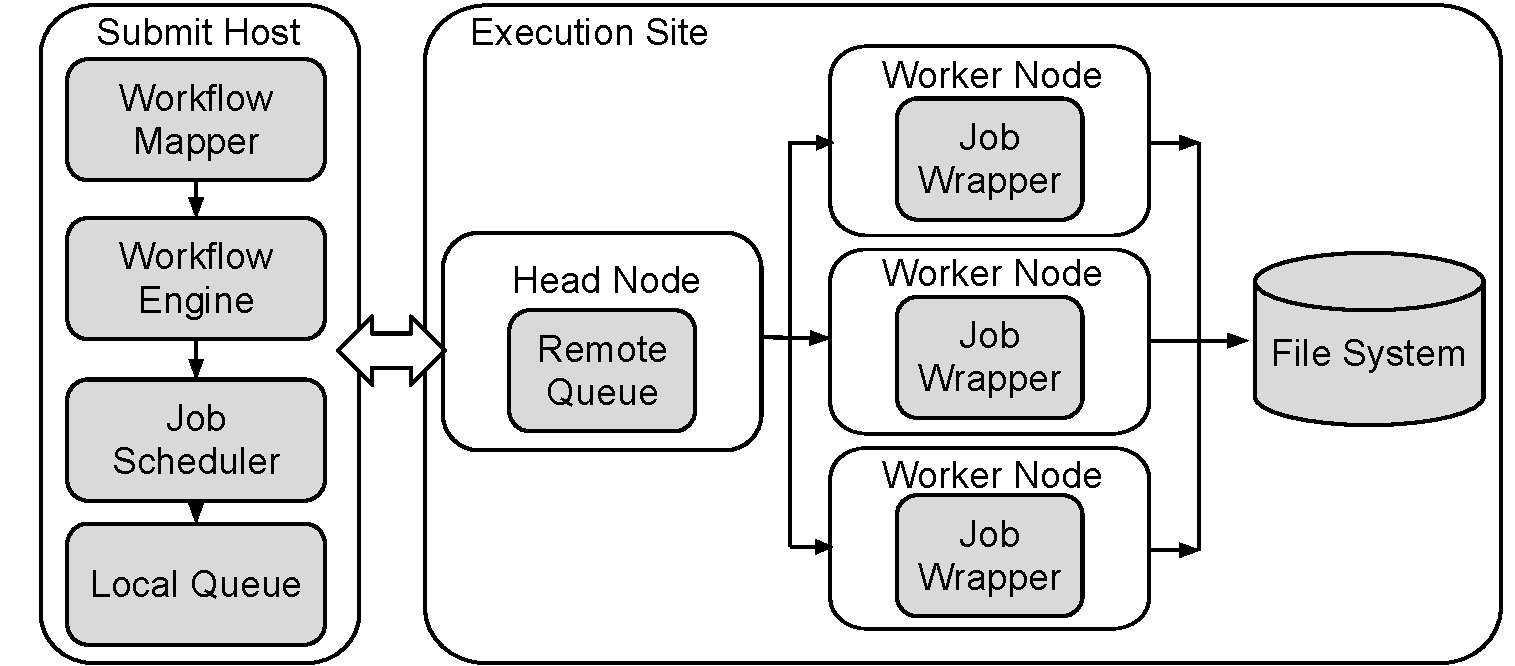
\includegraphics[width=.95\linewidth]{model}
	\caption{Overview of the workflow management system.}
	\label{fig:model-system}
	\vspace{-15pt}
\end{figure}

\vspace{4pt}
\noindent \textbf{Workflow Mapper.} Generates an executable workflow from an abstract 
workflow~\cite{Deelman2005} provided by the user or a workflow composition system. It restructures 
the workflow for performance optimization, and adds tasks for data management and provenance 
information generation. In this work, the workflow mapper is also used to merge fine-grained tasks into
a single clustered job (i.e., \emph{task clustering}). A job then is a single execution unit in the workflow 
execution systems and is composed of one or more tasks. 

\vspace{4pt}
\noindent \textbf{Workflow Engine.} Executes jobs defined by the workflow in order of their 
dependencies. Only jobs that have all their parent jobs completed are submitted to the Job 
Scheduler. The workflow engine relies on the resources (compute, storage, and network) 
defined in the executable workflow to perform computations. The elapsed time from when a 
job is released (all of its parents have completed successfully) to when it is submitted to the 
job scheduler is denoted as the workflow engine delay.

\vspace{4pt}
\noindent \textbf{Job Scheduler and Local Queue.} Manage individual workflow jobs and 
supervise their execution on local and remote resources. The elapsed time from when a 
task is submitted to the job scheduler to when it starts its execution in a worker node is 
denoted as the queue delay. It reflects both the efficiency of the job scheduler and the 
resource availability. 

\vspace{4pt}
\noindent \textbf{Job Wrapper.} Extracts tasks from clustered jobs and executes them at 
the worker nodes. The clustering delay is the elapsed time of the extraction process.

We extend the DAG model to be overhead aware (o-DAG). System overheads play an 
important role in workflow execution and constitute a major part of the overall runtime when 
tasks are poorly clustered~\cite{Chen2011}. Fig.~\ref{fig:model-odag} shows how we augment 
a DAG to be an o-DAG with the capability to represent system overheads ($s$) such as the 
workflow engine and queue delays. In addition, system overheads also include data transfer 
delay caused by staging-in and staging-out data. This classification of system overheads is 
based on our prior study on workflow analysis~\cite{Chen2011}. 

\begin{figure}[!t]
	\centering
	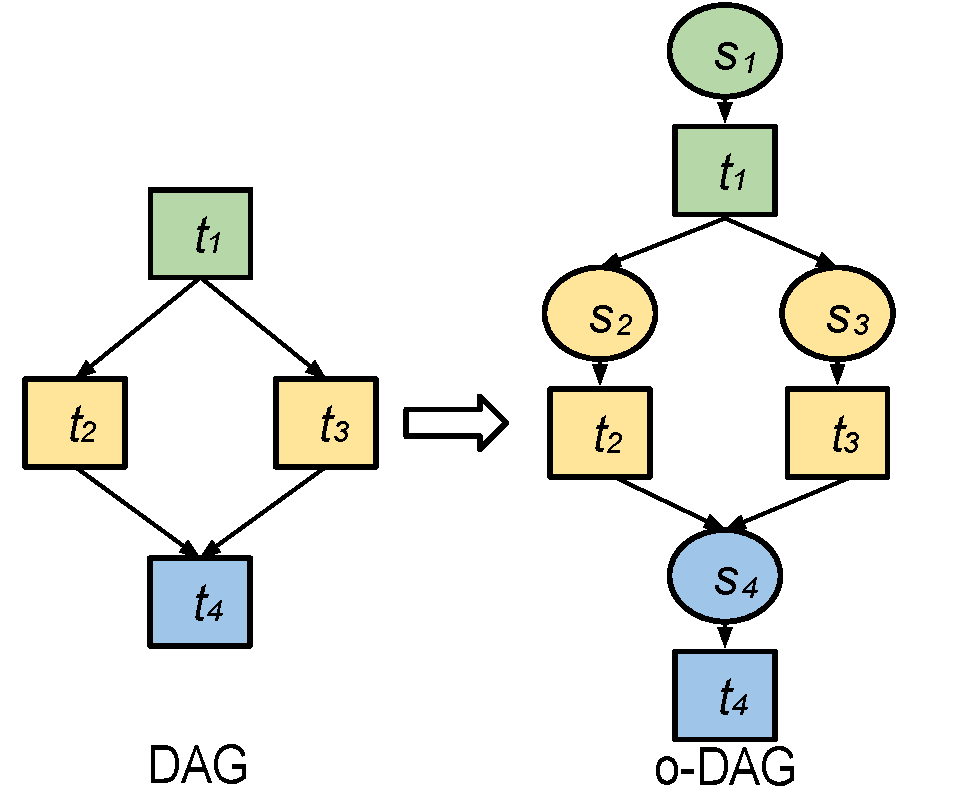
\includegraphics[width=0.6\linewidth]{odag.pdf}
	\captionof{figure}{Extending DAG to o-DAG ($s$ denotes a system overhead).}
	\label{fig:model-odag}
	\vspace{-15pt}
\end{figure}

With an o-DAG model, we can explicitly express the process of task clustering. In this work, we 
address task clustering horizontally and vertically. \textbf{Horizontal Clustering} (HC) merges 
multiple tasks within the same horizontal level of the workflow---the horizontal level of a 
task is defined as the longest distance from the DAG's entry task to this task. \textbf{Vertical 
Clustering} (VC) merges tasks within a pipeline of the workflow. Tasks at the same pipeline share 
a \emph{single-parent-single-child} relationship, i.e. a task $t_b$ has a unique parent $t_a$, which 
has a unique child $t_b$.

Fig.~\ref{fig:model-hc} shows a simple example on how to perform HC, in which two tasks $t_2$ 
and $t_3$, without data dependency between them, are merged into a clustered job $j_1$. Job 
wrappers are commonly used to execute clustered jobs, but they add an overhead denoted by the 
clustering delay $c$. The clustering delay measures the difference between the sum of the actual 
task runtimes and the job runtime seen by the job scheduler. After horizontal clustering, $t_2$ and 
$t_3$ in $j_1$ can be executed in sequence or in parallel, if parallelism is supported. In this work, 
we consider sequential executions only. Given a single resource, the overall runtime for the workflow 
in Fig.~\ref{fig:model-hc} (left) is $runtime_l= \sum_{i=1}^{4}(s_i+t_i)$, and the overall runtime for the 
clustered workflow in Fig.~\ref{fig:model-hc} (right) is $runtime_r=s_1+t_1+s_2+c_1+t_2+t_3+s_4+t_4$.  
$runtime_l > runtime_r$ as long as $c_1 < s_3$, which is often the case in many distributed systems 
since the clustering delay within a single execution node is usually shorter than the scheduling overhead 
across different execution nodes. 

\begin{figure}[b]
\centering
 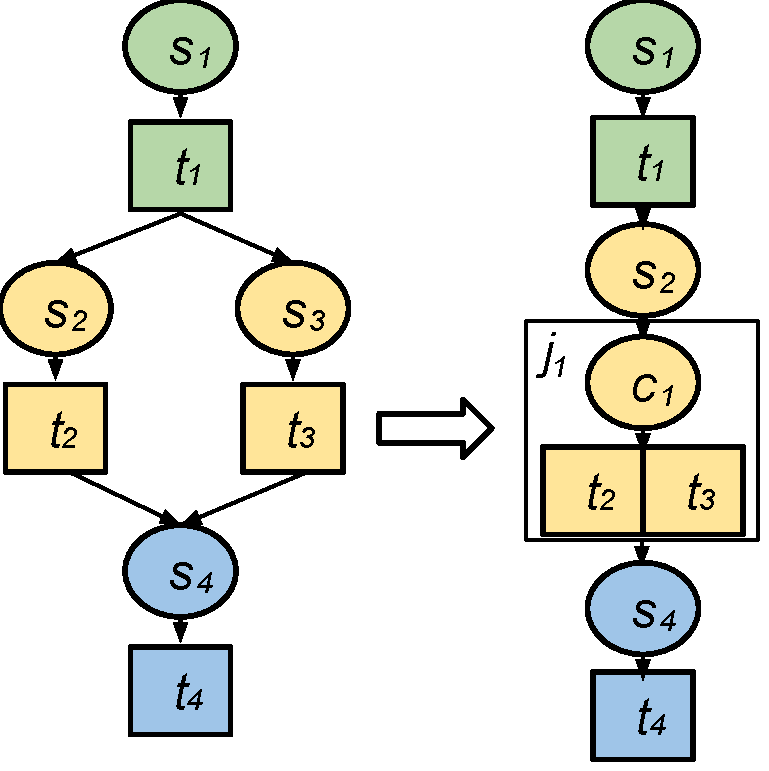
\includegraphics[width=0.45\linewidth]{hc.pdf}
  \captionof{figure}{A simple example of horizontal clustering (color indicates the horizontal level of a task).}
  \label{fig:model-hc}
\end{figure}

\begin{figure}[!htb]
\centering
 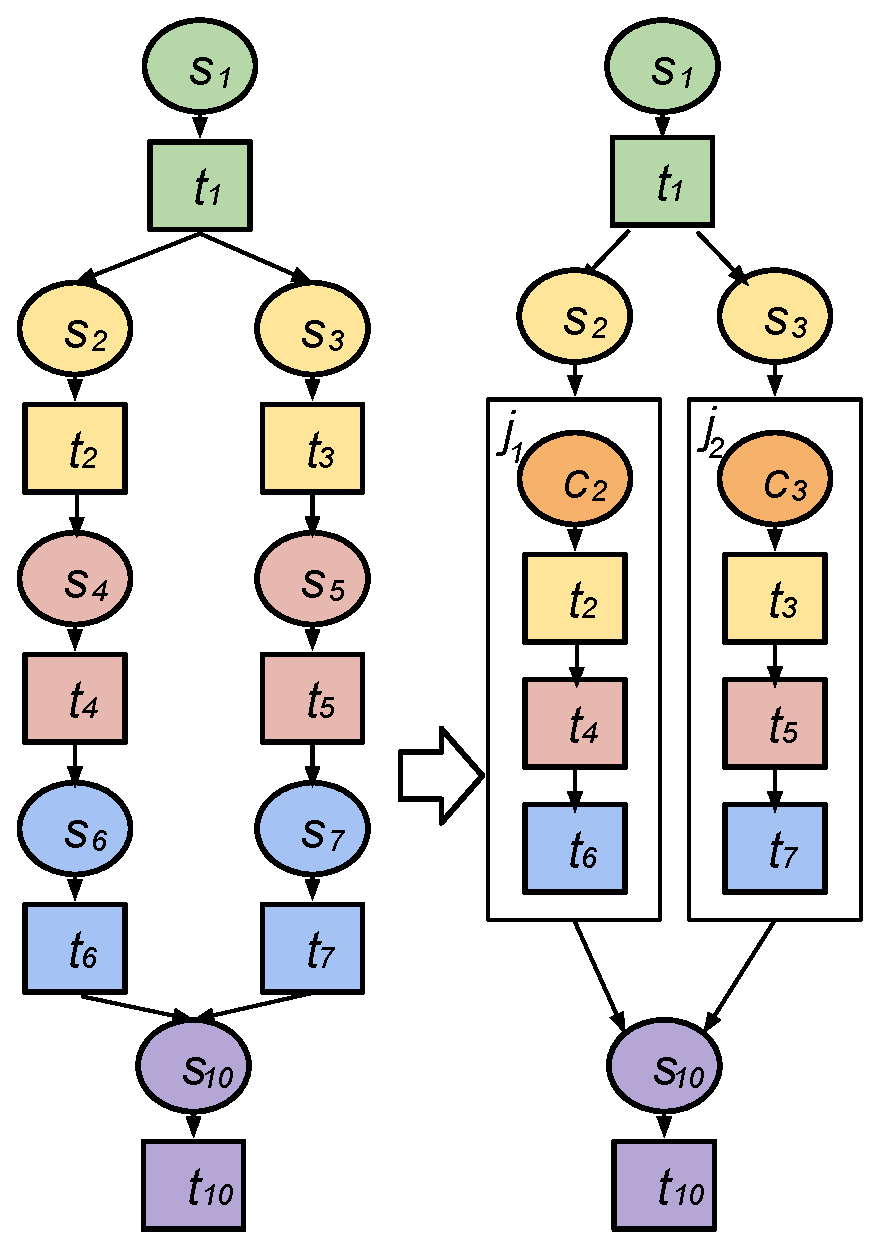
\includegraphics[width=0.5\linewidth]{vc.pdf}
  \captionof{figure}{A simple example of vertical clustering.}
  \label{fig:model-vc}
  \vspace{-15pt}
\end{figure}

Fig.~\ref{fig:model-vc} illustrates an example of vertical clustering, in which tasks $t_2$, $t_4$, 
and $t_6$ are merged into $j_1$, while tasks $t_3$, $t_5$, and $t_7$ are merged into $j_2$. 
Similarly, clustering delays $c_2$ and $c_3$ are added to $j_1$ and $j_2$ respectively, but 
system overheads $s_4$, $s_5$, $s_6$, and $s_7$ are removed. 

On situations where the scheduling and queue overheads are important, the use of task clustering 
techniques can significantly improve the workflow execution performance. In an ideal scenario, where
failures are absent, the number of tasks in a clustered job (clustering size, $k$) would be defined
as the number of all tasks in the queue divided by the number of available resources. Such a na\"{i}ve 
setting assures that the number of jobs is equal to the number of resources and the workflow can 
fully utilize the resources. However, in a faulty environment the clustering size should be defined
according to the failure rates, in particular, the task failure rate. Intuitively speaking, if the task failure 
rate is high, the clustered jobs may need to be re-executed more often compared to the case without 
clustering. Such performance degradation will counteract the benefits of reducing scheduling overheads. 
In the rest of this work, we will show how to adjust $k$ based on the estimated parameters of the task 
runtime $\bm t$, the system overhead $\bm s$, and the inter-arrival time of task failures $\bm\gamma$. 



\subsection{Task Failure Model}
\label{sec:task-failure-model}

In our prior work~\cite{Chen2011}, we have verified that system overheads $s$ better fits a Gamma or 
a Weibull distribution rather than an Exponential or Normal distribution. Schroeder et al.~\cite{Schroeder2006} 
have verified that the inter-arrival time of task failures fits a Weibull distribution with a shape parameter 
of 0.78, which fits better than the Lognormal and Exponential distributions. In~\cite{McConnel}, transient 
errors also follow a Weibull distribution. In~\cite{Sun2003, Iosup2008}, Weibull, Gamma and Lognormal 
distributions are among the best fit to estimate task runtimes for a set of workflow traces. Without loss of 
generality, we choose the Gamma distribution to model the task runtime~($\bm t$) and the system 
overhead ($\bm s$), and the Weibull distribution to model the inter-arrival time of failures ($\bm\gamma$). 
$\bm s$, $\bm t$ and $\bm \gamma$ are random variables of all tasks instead of one specific task. 


% We will reuse this shape parameter of 0.78 in our failure model. 

Probability distributions such as Weibull and Gamma are usually described with two parameters: the 
\emph{shape parameter}~($\phi$) and the \emph{scale parameter}~($\theta$). The shape parameter 
affects the shape of a distribution, while the scale parameter affects the stretching or shrinking of a 
distribution. Both parameters control the characteristics of a distribution. For example, the mean of a 
Gamma distribution is $\phi\theta$ and the Maximum Likelihood Estimation (MLE) is $(\phi-1)\theta$. 

Let $a$, $b$ be the parameters of the prior knowledge, $D$ the observed dataset, and $\theta$ the 
parameter we aim to estimate. In Bayesian probability theory, if the posterior distribution $p(\theta|D, a, b)$ 
is in the same family as the prior distribution $p(\theta|a, b)$, the prior and the posterior distributions 
are then called conjugate distributions, and the prior is called a conjugate prior for the likelihood 
function~\cite{diaconis1979conjugate}. For example, the Inverse-Gamma family is conjugate to itself 
(or self-conjugate) with respect to a Weibull likelihood function: if the likelihood function is Weibull, 
choosing an Inverse-Gamma prior over the mean will ensure that the posterior distribution is also 
Inverse-Gamma. Based on this definition, the parameters estimation of our task failure model has 
its foundations on prior works on failure and performance analyzes~\cite{Schroeder2006, Iosup2008, 
Sun2003, Chen2011}.

Therefore, once observed data $D$, the posterior distribution of $\theta$ is determined as follows:

\begin{eqnarray}
	\displaystyle  
	p(\theta|D, a, b)&=&\frac{p(\theta|a, b)\times p(D|\theta)}{p(D|a, b)}\nonumber  \\
	&\propto&p(\theta|a, b)\times p(D|\theta)
\end{eqnarray}
where $D$ is the observed inter-arrival time of failures~$X$, the observed task runtime~$RT$, 
or the observed system overheads~$S$; $p(\theta|D,a, b)$ is the posterior we aim to compute; 
$p(\theta|a, b)$ is the prior, which we already known from previous works; and $p(D|\theta)$ is 
the likelihood. We define $X=\{x_1, x_2, \dots, x_n\}$ as the observed data of the inter-arrival time 
of failures~$\bm\gamma$ during the execution. Similarly, we define $RT=\{t_1, t_2, \dots, t_n\}$ 
and  $S=\{s_1, s_2, \dots, s_n\}$ as the observed data of task runtime~$\bm t$ and system 
overheads~$\bm s$ respectively.  

More specifically, we model the inter-arrival time of failures ($\bm\gamma$) with a Weibull distribution 
as in~\cite{Schroeder2006}, which has a known shape parameter of~$\phi_{\gamma}$ and an 
unknown scale parameter~$\theta_{\gamma}$: $\bm\gamma\sim W(\theta_{\gamma}, \phi_{\gamma})$. 

The conjugate pair of a Weibull distribution with a known shape parameter~$\phi_{\gamma}$ is an 
Inverse-Gamma distribution, which means if the prior distribution follows an Inverse-Gamma 
distribution $\Gamma^{-1}(a_{\gamma}, b_{\gamma})$ with the shape parameter as~$a_{\gamma}$ 
and the scale parameter as $b_{\gamma}$, then the posterior follows an Inverse-Gamma distribution
as follows:

\begin{equation}
	\theta_{\gamma}\sim\Gamma^{-1}(a_{\gamma}+n,\displaystyle b_{\gamma}+\sum_{i=1}^n{x_i^{\phi_{\gamma}}})
	\label{eq:theta-1}
 \end{equation}

The MLE (Maximum Likelihood Estimation) of the scale parameter $\theta_{\gamma}$ is defined as:

\begin{equation}
	MLE(\theta_{\gamma})=\displaystyle\frac{b_{\gamma}+\displaystyle\sum_{i=1}^n{x_i^{\phi_{\gamma}}}}{a_{\gamma}+n+1}
\end{equation}
The understanding of the MLE is two fold: in the initial case there is no data, thus the MLE is determined
by the prior knowledge, i.e. $\displaystyle\frac{b_{\gamma}}{a_{\gamma}+1}$; when $n~\to~\infty$, the 
MLE $\displaystyle\frac{\displaystyle\sum_{i=1}^n{x_i^{\phi_{\gamma}}}}{n+1}\to\overline{x^{\phi_{\gamma}}}$, 
which means it is determined by the observed data, and is close to the regularized average of the observed 
data. If the estimation process only utilizes the prior knowledge, it is named \textbf{Static Estimation}. If the
process utilizes both the prior and posterior knowledge, it is named \textbf{Dynamic Estimation}.

We model the task runtime ($\bm t$) with a Gamma distribution as in~\cite{Sun2003, Iosup2008}, 
with a known shape parameter~$\phi_{t}$ and an unknown scale parameter~$\theta_t$. The 
conjugate pair of Gamma distribution with a known shape parameter is also a Gamma distribution. 
If the prior knowledge follows $\Gamma(a_t, b_t)$, where $a_t$ is the shape parameter and 
$b_t$ the rate parameter (or $\displaystyle \tfrac{1}{b_t}$ is the scale parameter), the posterior 
follows $\Gamma(a_t+n\phi_t, b_t+\displaystyle\sum_{i=1}^n{t_i})$ with $a_t+n\phi_t$ as the 
shape parameter and $b_t+\displaystyle\sum_{i=1}^n{t_i}$ as the rate parameter. The MLE of 
$\theta_t$ is then defined as follows: 

\begin{equation}
	MLE(\theta_t) = \displaystyle\frac{b_t+\displaystyle\sum_{i=1}^n{t_i}}{a_t+n\phi_t-1}
\end{equation}
	
Similarly, if we model the system overhead~$\bm s$ with a Gamma distribution with a known 
shape parameter $\phi_{s}$ and an unknown scale parameter $\theta_s$, and the prior knowledge 
as $\Gamma(a_s, b_s)$, the MLE of $\theta_s$ is thus defined as follows:

\begin{equation}
	MLE(\theta_s) = \displaystyle\frac{b_s+\displaystyle\sum_{i=1}^n{s_i}}{a_s+n\phi_s-1}
\end{equation}

We have assumed the task runtime, system overheads, and inter-arrival time between failures 
are a function of task types. The reason is that tasks at different levels (the deepest depth from 
the entry task to this task) are often of different types (a.k.a. transformations) in scientific 
workflows. Given $n$ independent tasks at the same workflow level and the distribution of the 
task runtime, the system overheads, and the inter-arrival time of failures, we aim at reducing the 
overall runtime $\bm M$ for completing these tasks by adjusting the clustering size $k$ (the 
number of tasks in a job). $\bm M$ is also a random variable, which includes the system overheads 
and the runtime of the clustered job and its subsequent retried jobs if the first attempt fails. We also 
assume that task failures are independent for each worker node (but with the same distribution) 
without considering the failures that bring the whole system down (e.g. a failure in the shared file 
system). 

The runtime of a job is a random variable indicated by $\bm d$. A clustered job succeeds only if 
all of its tasks succeed. The job runtime is the sum of the cumulative task runtime of $k$ tasks 
and the system overhead. We assume that the task runtime of each task is independent of each 
other, therefore the cumulative task runtime of $k$ tasks is also a Gamma distribution since the 
sum of Gamma distributions with the same scale parameter is still a Gamma distribution. We also 
assume the system overhead is independent of all the task runtimes. A general solution to express 
the sum of independent Gamma distributions with different scale and shape parameters is provided 
in~\cite{nadarajah2008review}. For simplicity, we limit this work to show a typical case where the 
system overhead and the task runtime have the same scale parameter ($\theta_{ts}=\theta_{t}=\theta_{s}$). 

Therefore, the job runtime (regardless of whether it succeeds of fails) is defined as follows:
\begin{eqnarray}
	\displaystyle
	\bm{d}\sim\Gamma(k\phi_{t}+\phi_{s}, \theta_{ts})\\
	MLE(\bm{d})=\displaystyle{(k\phi_t+\phi_s - 1) }{\theta_{ts}}
	\label{eq:N}
\end{eqnarray}

%We assume that $n \gg r$, but $n/k$ is not necessarily much larger than $r$ since $k$ could be very large. Normally at the beginning of workflow execution, $n/k > r$, which means there are more clustered jobs than available resources. To try all $n$ tasks once, irrespective of whether they succeed or fail, one needs approximately $\displaystyle \frac{n}{rk}$ execution cycle(s) since at each execution cycle we can execute at most $r$ jobs. Therefore, 

%We have assumed the task runtime $t\sim\Gamma^{-1}(a_t, b_t)$. $(a_t, b_t)$ are estimated from prior knowledge and/or posterior knowledge. The system overhead $s\sim\Gamma^{-1}(a_s, b_s)$ similarly. By merging the $k$ tasks together, their computational runtime still follows a Inverse-Gamma distribution with parameter $(a_t, kb_t)$. We use $\mathcal{L}(f)$ to indicate the Laplace transform of the distribution $f$ (time-series signal in Laplace transform). $d$ is a random variable that represents the job runtime, which includes the computational runtime of $k$ tasks and the system overhead $s$. The PDF of $d$ is: $M$ is a random variable represents the cumulative job runtime of $\displaystyle\frac{n}{k}$ jobs. For a given $M$, we have:

Let $N$ be the retry time of clustered jobs. The process to run and retry a job is a Bernoulli trial 
with exactly two possible outcomes: \emph{success} or \emph{failure}. Once a job fails, it will be 
re-executed until it is eventually successfully executed (since failures are assumed transient). 
For a given job runtime $d_i$, the retry time $N_i$ of a clustered job $i$ is defined as follows:
\begin{eqnarray}
	\displaystyle
	N_i=\frac{1}{1-F(d_i)}=\frac{1}{e^{-\left(\displaystyle\frac{d_i}{\theta_{\gamma}}\right)^{\phi_{\gamma}}}}=e^{\left(\displaystyle\frac{d_i}	{\theta_{\gamma}}\right)^{\phi_{\gamma}}} 
	\label{eq:N}
\end{eqnarray}
where $F(d_i)$ is the CDF (Cumulative Distribution Function) of $\bm\gamma$. The time to 
complete $d_i$ successfully in a faulty execution environment is determined as follows:
\begin{eqnarray}
	\displaystyle
	M_i=d_i \times N_i=d_i \times e^{\left(\displaystyle\frac{d_i}{\theta_{\gamma}}\right)^{\phi_{\gamma}}} 
	\label{eq:M}
\end{eqnarray}

\noindent Equation \ref{eq:M} has involved two distributions $\bm d$ and $\theta_{\gamma}$ 
($\phi_{\gamma}$ is known). From Equation \ref{eq:theta-1}, we have:
\begin{eqnarray}
	\displaystyle\cfrac{1}{\theta_{\gamma}}\sim\Gamma\left(a_{\gamma}+n,\frac{1}{\displaystyle b_{\gamma}+\sum_{i=1}^n{x_i^{\phi_{\gamma}}}}\right) \\
	MLE\left(\displaystyle\cfrac{1}{\theta_{\gamma}}\right)=\displaystyle\cfrac{a_{\gamma}+n-1}{\displaystyle b_{\gamma}+\sum_{i=1}^n{x_i^{\phi_{\gamma}}}}
	\label{eq:theta}
 \end{eqnarray}

\noindent $M_i$ is a monotonic increasing function of both $d_i$ and $\displaystyle\cfrac{1}{\theta_{\gamma}}$, 
and the two random variables are independent of each other, therefore:
\begin{equation} 
	MLE(M_i)=MLE(d_i)e^{\left(\displaystyle MLE(d_i)MLE\left(\cfrac{1}{\theta_{\gamma}}\right)\right)^{\phi_{\gamma}}} 
	\label{eq:MLE-M-i}
\end{equation}

From Equation \ref{eq:MLE-M-i}, to attain $MLE(M_i)$ we just need to attain $MLE(d_i)$ and 
$MLE\left(\tfrac{1}{\theta_{\gamma}}\right)$ at the same time. In both dimensions ($d_i$ and 
$\displaystyle\tfrac{1}{\theta_{\gamma}}$), $M_i$ is a Gamma distribution, and each $M_i$ 
has the same distribution parameters, therefore:
\begin{eqnarray} 
	\label{eq:MLE-M}
	\bm{M}&=&\displaystyle\cfrac{1}{r} \times \sum_{i=1}^{\cfrac{n}{k}}M_i\sim\Gamma \nonumber\\
	MLE(\bm{M})&=&\displaystyle\cfrac{n}{rk} \times MLE(M_i)\\
	&=&\displaystyle\frac{n}{rk} \times MLE(d_i)e^{\left(\displaystyle MLE(d_i)MLE\left(\tfrac{1}{\theta_{\gamma}}\right)\right)^{\phi_{\gamma}}} 
\end{eqnarray}
where $r$ is the number of resources. 

In this work, we consider a compute cluster as a homogeneous cluster, which is often the case 
in dedicated clusters and cloud platforms. 

%On the other side, at the end of the workflow execution, since n is decreasing with the process of workflow, it is possible that $\displaystyle \frac{n}{k} < r$, which means there are fewer jobs than the available resources. One needs just one execution cycle to execute these tasks once. The time to complete all $n$ tasks successfully is $N(kt+s)$. 

%In summary, the estimated overall runtime is, 

%\begin{equation} 
%\label{eq:jfm}
%M=
%\begin{cases}
%\cfrac{n(kt+s)}{rk}{e^{(\cfrac{kt+s}{\theta})^{\phi}}}, & \text{if } \cfrac{n}{k}\geq r \\
%(kt+s){e^{(\cfrac{kt+s}{\theta})^{\phi}}}, & \text{else}
%\end{cases}
%\end{equation}

Let $k^*$ be the optimal clustering size that minimizes Equation~\ref{eq:MLE-M}. $\arg min$  
stands for the argument ($k$) of the minimum\footnote{http://en.wikipedia.org/wiki/Arg\_max}, 
i.e., the value of $k$ such that $MLE(\bm{M})$ attains its minimum value:
\begin{eqnarray} 
	\label{eq:k_optimal}
	k^*=\arg min\{MLE(\bm{M})\} 
\end{eqnarray}

\begin{figure}[b]
	\centering
	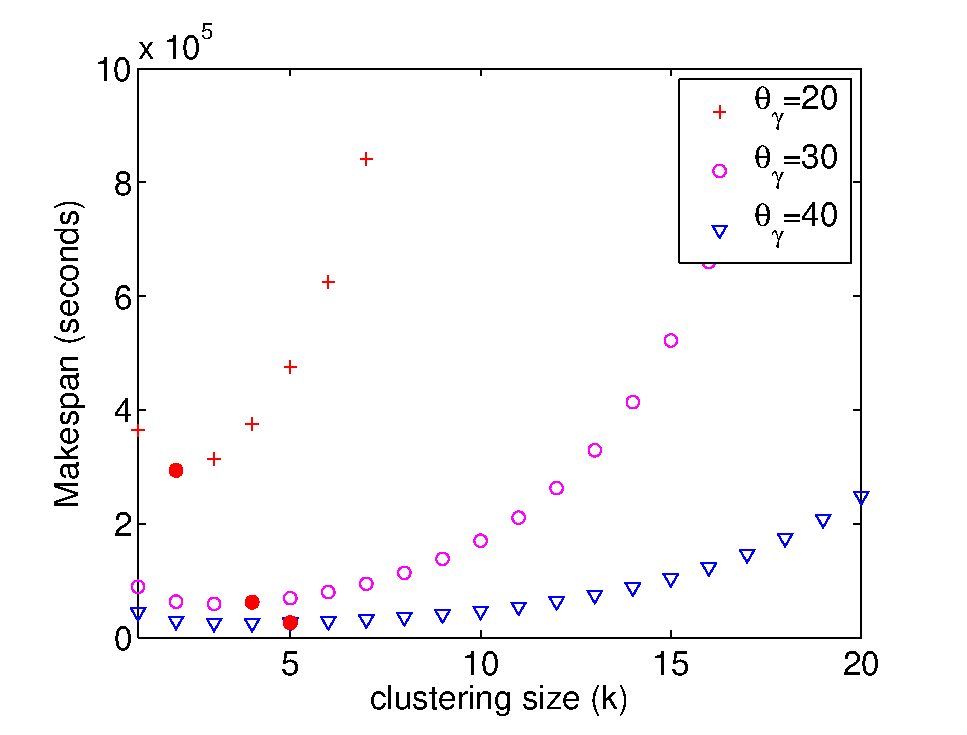
\includegraphics[width=0.8\linewidth]{model_makespan2.eps}
	\caption{Makespan with different clustering size and $\theta_{\gamma}$. ($n=1000$, $r=20$, $\phi_t=5$s, $\phi_s=50$s). Red dots are the minimums.}
	\label{fig:model-makespan}
\end{figure}

\begin{figure}[t]
	\centering
	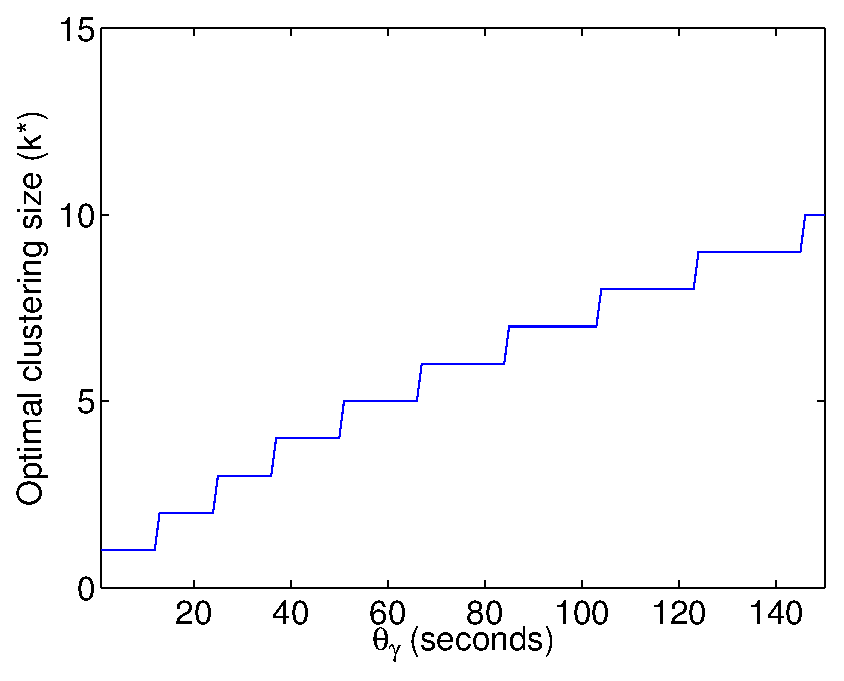
\includegraphics[width=0.8\linewidth]{model_size2.eps}
	\caption{Optimal clustering size ($k^*$) with different  $\theta_{\gamma}$ ($n=1000$, $r=20$, $\phi_t=5$s, $\phi_s=50$s).}
	\label{fig:model-size}
	\vspace{-15pt}
\end{figure}

It is difficult to find a analytical solution of $k^*$. However, there are a few constraints that can 
simplify the estimation of $k^*$: (\emph{i}) $k$ can only be an integer in practice; (\emph{ii}) 
$MLE(\bm{M})$ is continuous and has one minimum. Methods such as Newton's method can be 
used to find the minimal $MLE(\bm{M})$ and the corresponding $k$. Fig.~\ref{fig:model-makespan} 
shows an example of $MLE(\bm{M})$ using static estimation with a low task failure rate ($\theta_{\gamma}=40$s), 
a medium task failure rate ($\theta_{\gamma}=30$s) and a high task failure rate ($\theta_{\gamma}=20$s). 
Other parameters are $n=50$, $\phi_{t}=5$s and $\phi_{s}=50$s, and the scale parameter $\theta_{ts}$ is 
defined as 2 for simplicity. These parameters are close to the parameters of tasks at the level of 
the \texttt{mProjectPP} transformation of the Montage workflow (Section \ref{sec:experiments}).
Fig.~\ref{fig:model-size} shows the relationship between the optimal clustering size ($k^*$) and 
$\theta_{\gamma}$, which is a non-decreasing function. The optimal clustering size (red dots in 
Fig.~\ref{fig:model-makespan}) when $\theta_{\gamma} \in \{20,30,40\}$ is 2, 3, and 5 respectively. 
As expected, the longer the inter-arrival time of failures is, the lower the task failure rate is. With 
a lower task failure rate, a larger $k$ value assures that system overheads are reduced without 
retrying the tasks too many times.

From this theoretic analysis, we conclude that (\emph{i}) the longer the inter-arrival time of failures is, 
the better runtime performance the task clustering has; and (\emph{ii}) by adjusting the clustering 
size according to the inter-arrival time, the overall runtime performance can be improved. 

\begin{table}[!htb]
	\setlength{\tabcolsep}{9pt}
	\centering
	\small
	\begin{tabular}{lrrrr}
		\hline
		Parameter	& Description	  \\
		\hline
		$t$, $s$, $d$ & distribution of task runtime, overhead, job runtime\\
		$\gamma$& distribution of the inter-arrival time of failures \\
		$\theta_{\gamma}$, $\phi_{\gamma}$  		&scale and shape parameters of $\gamma$		\\
		$\theta_{t}$, $\phi_{t}$  		&scale and shape parameters of $t$		\\
		$\theta_{s}$, $\phi_{s}$  		&scale and shape parameters of $s$		\\
		$a_{\gamma}$, $b_{\gamma}$ & prior knowledge of $\gamma$\\
		$a_{t}$, $b_{t}$ & prior knowledge of $t$\\
		$a_{s}$, $b_{s}$ & prior knowledge of $s$\\
		$k$& number of tasks in a job\\
		$N$& distribution of the retry time of clustered jobs\\
		$N_i$& retry time of job $i$\\
		$M$ & distribution of the overall runtime \\
		$M_i$ & the overall runtime to complete job $i$\\
		$r$ & the number of available worker nodes\\
		$n$ & the number of tasks\\
		\hline
	\end{tabular}
	\caption{Explanation of the symbols used in this work.}
	\label{tab:model-variables}
	\vspace{-15pt}
\end{table} 

%
% Section: Fault-Tolerant Clustering
%
\section{Fault-Tolerant Clustering}
\label{sec:clustering}

Inappropriate task clustering may negatively impact the workflow makespan in faulty distributed
environments. In this section, we propose three fault-tolerant task clustering methods---Selective 
Reclustering (\emph{SR}), Dynamic Reclustering (\emph{DR}), and Vertical Reclustering 
(\emph{VR})---that adjust the clustering size of the jobs to reduce the impact of task failures on the 
workflow execution. These methods are based on the Horizontal Clustering (HC)~\cite{Singh2008} 
technique that has been implemented and used in the Pegasus WMS~\cite{Deelman2005}.

\vspace{5pt}
\noindent \textbf{Horizontal Clustering} (\emph{HC}). 
Horizontal clustering merges multiple tasks within the same horizontal level of the workflow. The 
clustering granularity (number of tasks within a cluster) of a clustered job is controlled by the user, 
who defines either the number of tasks per clustered job (\emph{clusters.size}), or the number of 
clustered jobs per horizontal level of the workflow (\emph{clusters.num}). For simplicity, we set \emph{clusters.num} 
to be the same as the number of available resources. In our prior work~\cite{Chen2013a,Chen2013b}, 
we have evaluated the runtime performance with different clustering granularity. 
Algorithm~\ref{alg:evaluation-hc} shows the pseudocode for HC. The \texttt{Clustering} and \texttt{Merge} 
procedures are called in the initial task clustering process, while the \texttt{Reclustering} procedure is 
invoked when a failed job is detected by the monitoring system. Fig.~\ref{fig:clustering-hc} shows an 
example where the initial clustering size is 4. As a result,  there are four tasks in a clustered job. 
During execution, three out of these tasks ($t_1$, $t_2$, $t_3$) fail. Due to the lack of an adaptive 
mechanism, HC keeps retrying all of the four tasks in the following attempts until all of them succeed.

\begin{algorithm}[t]
	\footnotesize
	\caption{Horizontal Clustering algorithm.}
	\label{alg:evaluation-hc}
	\begin{algorithmic}[1]
		\Require $W$: workflow; $C$: max number of tasks per job defined by \emph{clusters.size} or \emph{clusters.num}
		\Procedure{Clustering}{$W,C$}
			\For{$level < depth(W)$}
				\State $TL\gets $\ \Call{GetTasksAtLevel}{$W,level$} \Comment{Partition $W$ based on depth}
				\State $CL\gets$  \ \Call{Merge}{$TL,C$} \Comment{Returns a list of clustered jobs}
				\State $W \gets W - TL + CL$  \Comment{Merge dependencies as well} 
			\EndFor
		\EndProcedure
		\Procedure{Merge}{$TL, C$}
			\State $J\gets$ \{\}\Comment{An empty job}
			\State $CL\gets$\{\}\Comment{An empty list of clustered jobs}
			\While{$TL$ is not empty}
				\State $J$.add ($TL$.pop($C$) \Comment{Pops $C$ tasks that are not merged }
				\State  $CL$.add( $J$)
			\EndWhile
			\State \textbf{return} $CL$
		\EndProcedure
		\Procedure{Reclustering}{$J$}\Comment{$J$ is a failed job}
			\State $J_{new}\gets$\ \Call{CopyOf}{$J$} \Comment{Copy Job $J$}
			\State $W \gets W + J_{new}$ \Comment{Re-execute it}
		\EndProcedure
	\end{algorithmic}
\end{algorithm}

\begin{figure}[!t]
	\centering
	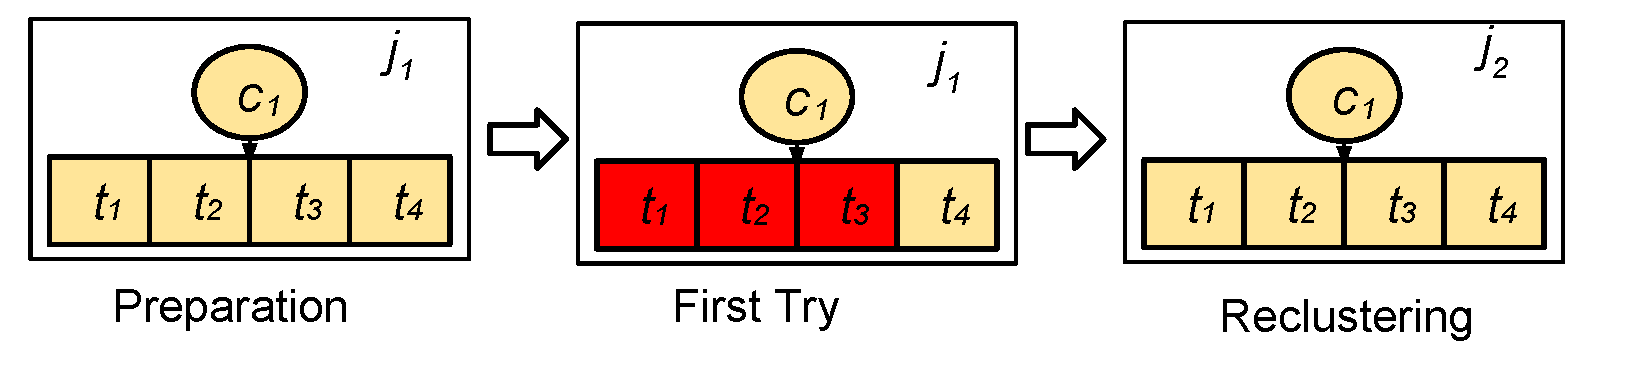
\includegraphics[width=0.85\linewidth]{hcr.pdf}
	\caption{An example of Horizontal Clustering (red boxes are failed tasks).}
	\label{fig:clustering-hc}
	\vspace{-15pt}
\end{figure}


\vspace{5pt}
\noindent \textbf{Selective Reclustering} (\emph{SR}).
The selective re-clustering technique, on the other hand, selects the failed tasks in a 
clustered job and merges them into a new clustered job. Algorithm~\ref{alg:evaluation-sr}
shows the pseudocode of the \texttt{Reclustering} procedure for the SR method. The 
\texttt{Clustering} and \texttt{Merge} procedures are the same as those for HC.
Fig.~\ref{fig:clustering-sr} shows an example of the SR method. In the first attempt, the 
clustered job, composed of 4 tasks,  has 3 failed tasks ($t_1$, $t_2$, $t_3$). Three failed 
tasks are merged into a new clustered job $j_2$ and retried. This approach does not intend 
to adjust the clustering size, although the clustering size will become smaller after each attempt 
since there are fewer tasks in subsequent clustered jobs. In the example, the clustering size 
has decreased from 4 to 3. However, the optimal clustering size may not be 3, which limits 
the workflow performance if the $\theta_{\gamma}$ is small and $k$ should be decreased 
as much as possible. The advantage of SR is that it is simple to implement and can be 
incorporated into existing workflow management systems with minimum impact on the 
workflow execution efficiency as shown in Section~\ref{sec:experiments}.

\begin{algorithm}[t]
	\footnotesize
	\caption{Selective Reclustering algorithm.}
	\label{alg:evaluation-sr}
	\begin{algorithmic}[1]
		\Require $W$: workflow; $C$: max number of tasks per job defined by \emph{clusters.size} or \emph{clusters.num}
			\Procedure{Reclustering}{$J$}\Comment{$J$ is a failed job}
			\State $TL \gets$\ \Call{GetTasks}{$J$}
			\State $J_{new}\gets$\{\}\Comment{An empty job}
			\ForAll{Task $t$ in $TL$}
				\If{$t$ is failed}
					\State $J_{new}$.add ($t$)
				\EndIf
			\EndFor
			\State $W \gets W + J_{new}$ \Comment{Re-execute it}
		\EndProcedure
	\end{algorithmic}
\end{algorithm}

\begin{figure}[!t]
	\centering
	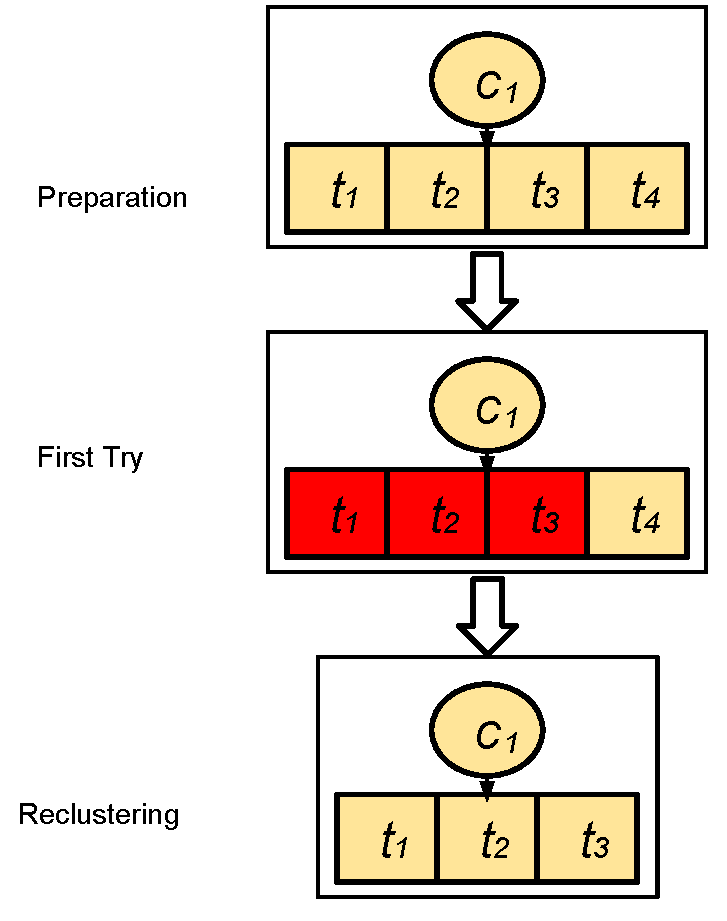
\includegraphics[width=0.78\linewidth]{sr.pdf}
	\caption{An example of Selective Reclustering (red boxes are failed tasks). Failed tasks are merged into a new job and retried.}
	\label{fig:clustering-sr}
	\vspace{-15pt}
\end{figure}

 \begin{figure}[b]
	\centering
	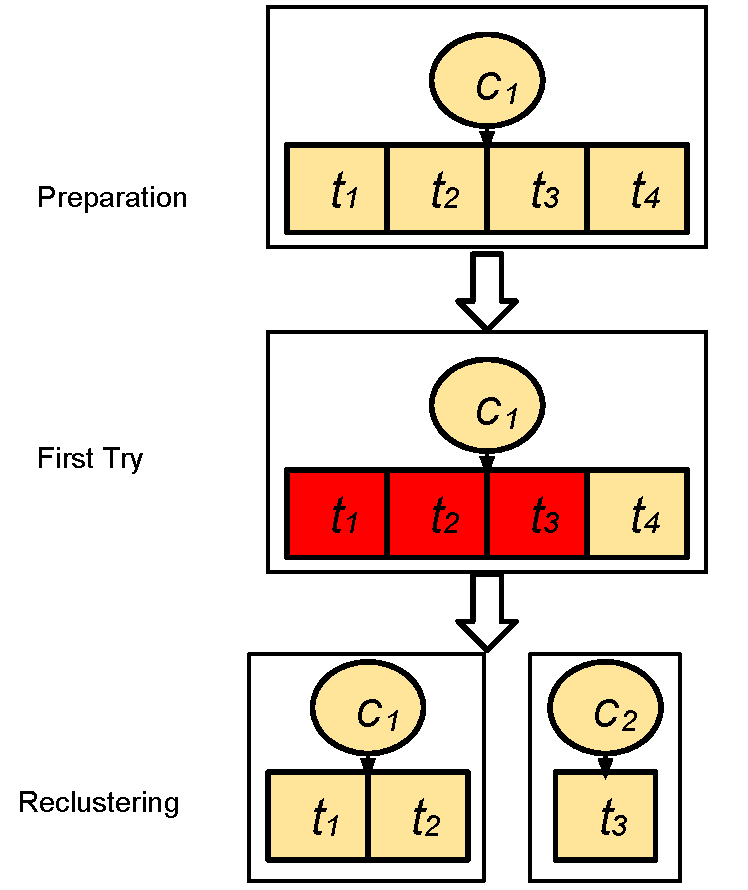
\includegraphics[width=0.73\linewidth]{dr.pdf}
	\caption{An example of Dynamic Reclustering (red boxes are failed tasks). The clustering size is adjusted to 2 and thus failed tasks are merged into two new clustered jobs.}
	\label{fig:clustering-dr}
	\vspace{-5pt}
\end{figure}

\vspace{5pt}
\noindent \textbf{Dynamic Reclustering} (\emph{DR}).
The Selective Reclustering method does not analyze the clustering size, rather it 
uses a self-adjusted approach to reduce the clustering size to the number of failed tasks. 
However, the actual optimal clustering size may be larger or smaller than the number of
failed tasks. Therefore, we propose the Dynamic Reclustering method that merges failed
tasks into new clustered jobs in which the clustering size is set to $k^*$ according to 
Equation~\ref{eq:k_optimal}. Algorithm~\ref{alg:evaluation-dr} shows the pseudocode 
for the \texttt{Reclustering} procedure for the DR method. Fig.~\ref{fig:clustering-dr} shows 
an example where the initial clustering size is 4 and thereby there are 4 tasks in the 
clustered job. In the first attempt, 3 tasks within the clustered job have failed. Therefore, 
there are only 3 tasks to be retried, and thus the clustering size should be decreased to 2 
accordingly. Two new clustered jobs $j_2$ (containing $t_1$ and $t_2$) and $j_3$ 
(containing $t_3$) are created. Reducing the granularity of failed clustered jobs may
decrease the probability of future failures, since at least one of the jobs will execute on
a different worker node.

\begin{algorithm}[t]
	\footnotesize
	\caption{Dynamic Reclustering algorithm.}
	\label{alg:evaluation-dr}
	\begin{algorithmic}[1]
		\Require $W$: workflow; $C$: max number of tasks per job defined by \emph{clusters.size} or \emph{clusters.num}
			\Procedure{Reclustering}{$J$}\Comment{$J$ is a failed job}
			\State $TL \gets$\ \Call{GetTasks}{$J$}
			\State $J_{new}\gets$\{\}
			\ForAll{Task $t$ in $TL$}
				\If{$t$ is failed}
					\State $J_{new}$.add ($t$)
				\EndIf
				\If{$J_{new}.size() > k^*$}
					\State $W \gets W + J_{new}$
					\State $J_{new}\gets$\{\}
				\EndIf
			\EndFor
			\State $W \gets W + J_{new}$ \Comment{Re-execute it}
		\EndProcedure
	\end{algorithmic}
\end{algorithm}

\begin{algorithm}[!t]
	\footnotesize
	\caption{Vertical Reclustering algorithm.}
	\label{alg:evaluation-vr}
	\begin{algorithmic}[1]
		\Require $W$: workflow; 
		\Procedure{Clustering}{$W$}
			\For{$level < depth(W)$}
				\State $TL\gets $\ \Call{GetTasksAtLevel}{$W,level$} \Comment{Partition $W$ based on depth}
				\State $CL, TL_{merged}\gets$  \ \Call{Merge}{$TL$} \Comment{Returns a list of clustered jobs}
				\State $W \gets W - TL_{merged} + CL$  \Comment{Merge dependencies as well} 
			\EndFor
		\EndProcedure
		\Procedure{Merge}{$TL$}
			\State $TL_{merged}\gets TL$\Comment{All the tasks that have been merged}
			\State $CL\gets$\{\}\Comment{An empty list of clustered jobs}
			\ForAll{$t$ in $TL$}
				\State $J\gets$ \{$t$\}
				\While{$t$ has only one child $t_{child}$ and $t_{child}$ has only one parent}
					\State $J$.add ($t_{child}$)
					\State $TL_{merged}\gets TL_{merged} + t_{child}$ 
					\State $t\gets t_{child}$
				\EndWhile
				\State  $CL$.add( $J$)
			\EndFor
			\State \textbf{return} $CL$, $TL_{merged}$
		\EndProcedure
		\Procedure{Reclustering}{$J$}\Comment{$J$ is a failed job}
			\State $TL \gets$\ \Call{GetTasks}{$J$}
			\State $k^*\gets J.size() / 2$ \Comment{Reduce the clustering size by half}
			\State $J_{new}\gets$\{\}
			\ForAll{Task $t$ in $TL$}
				\If{$t$ is failed or not completed}
					\State $J_{new}$.add ($t$)
				\EndIf
				\If{$J_{new}.size() > k^*$}
					\State $W \gets W + J_{new}$
					\State $J_{new}\gets$\{\}
				\EndIf
			\EndFor
			\State $W \gets W + J_{new}$ \Comment{Re-execute it}
		\EndProcedure
	\end{algorithmic}
\end{algorithm}

\begin{figure}[t]
\centering
  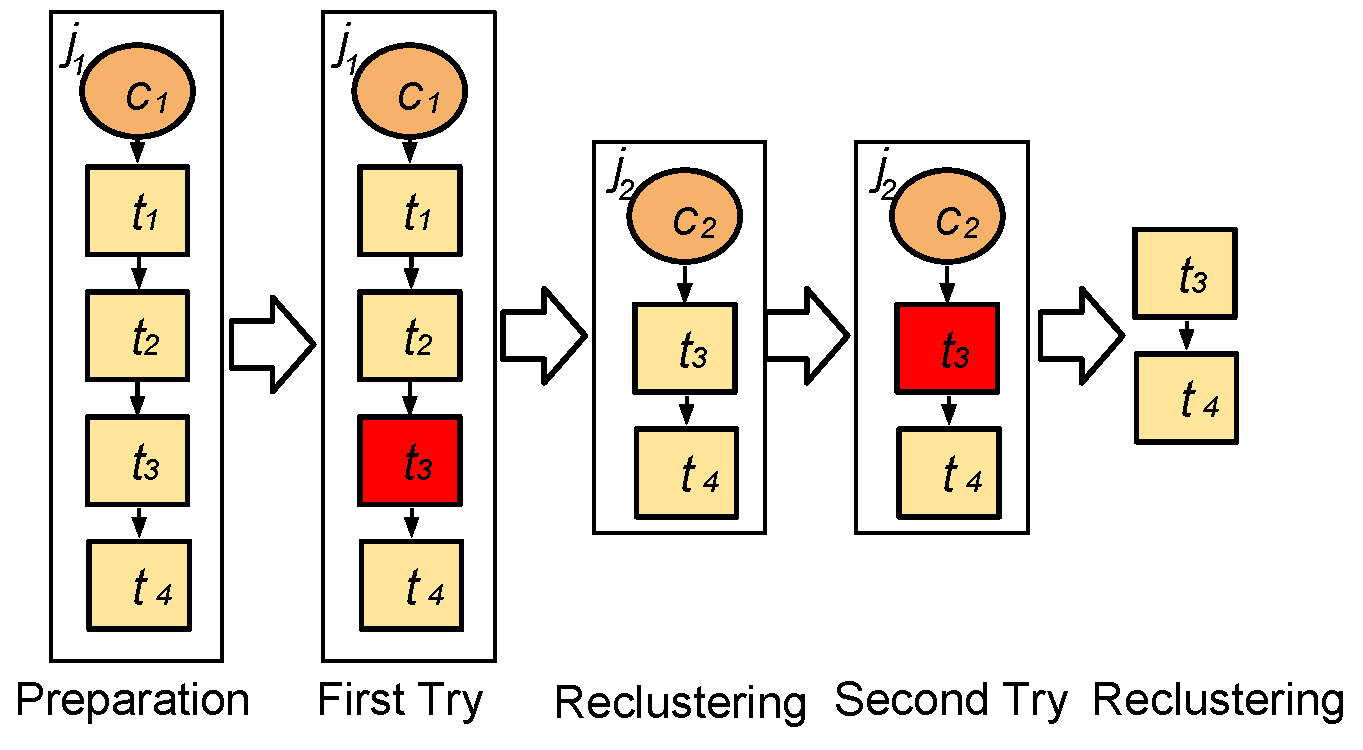
\includegraphics[width=0.8\linewidth]{vr.pdf}
  \caption{An example of Vertical Reclustering (red boxes are failed tasks). The clustering size is decreased by half when a job execution fails.}
  \label{fig:clustering-vr}
  \vspace{-15pt}
\end{figure}

\vspace{5pt}
\noindent \textbf{Vertical Reclustering} (\emph{VR}). VR is an extension of the Vertical 
Clustering (Section~\ref{sec:model}) method. Similar to Selective Reclustering, Vertical 
Reclustering only retries failed or not completed tasks. If a failure is detected, $k$ is
decreased by half and failed tasks are re-clustered accordingly. Fig.~\ref{fig:clustering-vr}
shows an example of VR where tasks within a pipeline are initially merged into a single 
clustered job ($t_1$, $t_2$, $t_3$, $t_4$). $t_3$ fails at the first attempt assuming it is 
a failure-prone task (i.e., its $\theta_{\gamma}$ is short). VR then retries only the failed task 
($t_3$) and tasks that have not been yet completed ($t_4$) by merging them into a new 
job $j_2$. In the second attempt, $j_2$ fails and then it is divided into two jobs containing one
task each ($t_3$ and $t_4$). Since the clustering size is already 1, VR performs no vertical 
clustering anymore and will continue retrying $t_3$ and $t_4$ (but still following their data 
dependency) until they succeed. Algorithm \ref{alg:evaluation-vr} shows the pseudocode 
for the VR method. 



%
% Section: Experiments and Discussions
%
\section{Experiments and Discussions}
\label{sec:experiments}

In this section, we evaluate our methods with five scientific workflow applications, whose 
runtime information is gathered from real execution traces. We conduct a simulation-based 
approach in which we vary system parameters such as the task failures inter-arrival time 
in order to evaluate the reliability of our fault-tolerant task clustering methods.


\subsection{Scientific Workflow Applications}
\label{sec:applications}

In the experiments, we use the following scientific workflow applications: LIGO Inspiral 
analysis, Montage, CyberShake, Epigenomics, and SIPHT. Below, we briefly describe 
each of them and present their main characteristics and structures:

\begin{figure}[b]
	\centering
	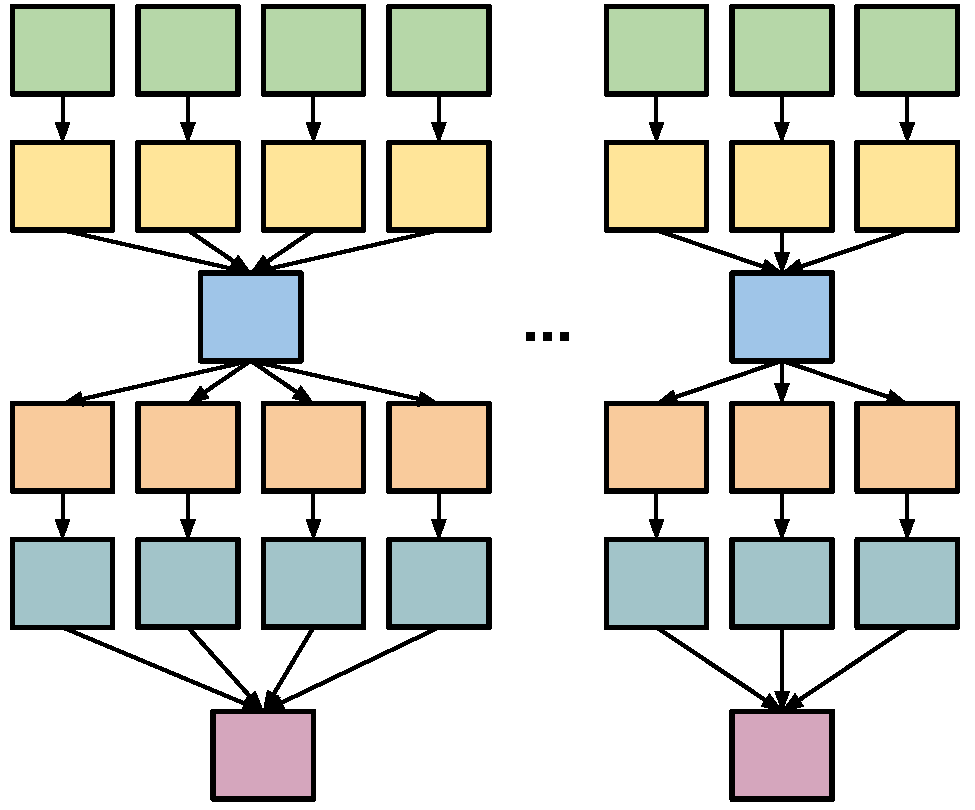
\includegraphics[width=0.5\linewidth]{ligo_shape.pdf} \\
	\caption{Simplified visualization of the LIGO workflow.}
	\label{fig:evaluation-shape-ligo}
	\vspace{-5pt}
\end{figure}

\noindent \textbf{LIGO.}
Laser Interferometer Gravitational Wave Observatory (LIGO)~\cite{LIGO} workflows are 
used to search for gravitational wave signatures in data collected by large-scale interferometers. 
The observatories' mission is to detect and measure gravitational waves predicted by general 
relativity (Einstein's theory of gravity), in which gravity is described as due to the curvature of 
the fabric of time and space. Fig.~\ref{fig:evaluation-shape-ligo} shows a simplified version of
the workflow. The LIGO Inspiral workflow is separated into multiple groups of interconnected 
tasks, which we call branches in the rest of this work. Each branch may have a different number 
of pipelines. The LIGO workflow is a data-intensive workflow.

\noindent \textbf{Montage.}
Montage~\cite{Berriman2004} is an astronomy application used to construct large image 
mosaics of the sky. Input images are reprojected onto a sphere and overlap is calculated for each 
input image. The application re-projects input images to the correct orientation while keeping 
background emission level constant in all images. Images are added by rectifying them to a 
common flux scale and background level. Finally the reprojected images are co-added into a final 
mosaic. The resulting mosaic image can provide a much deeper and detailed understanding of the 
portion of the sky in question. Fig.~\ref{fig:evaluation-shape-montage} illustrates a small Montage 
workflow. The size of the workflow depends on the number of images used in constructing the desired 
mosaic of the sky. 

\begin{figure}[!t]
	\centering
	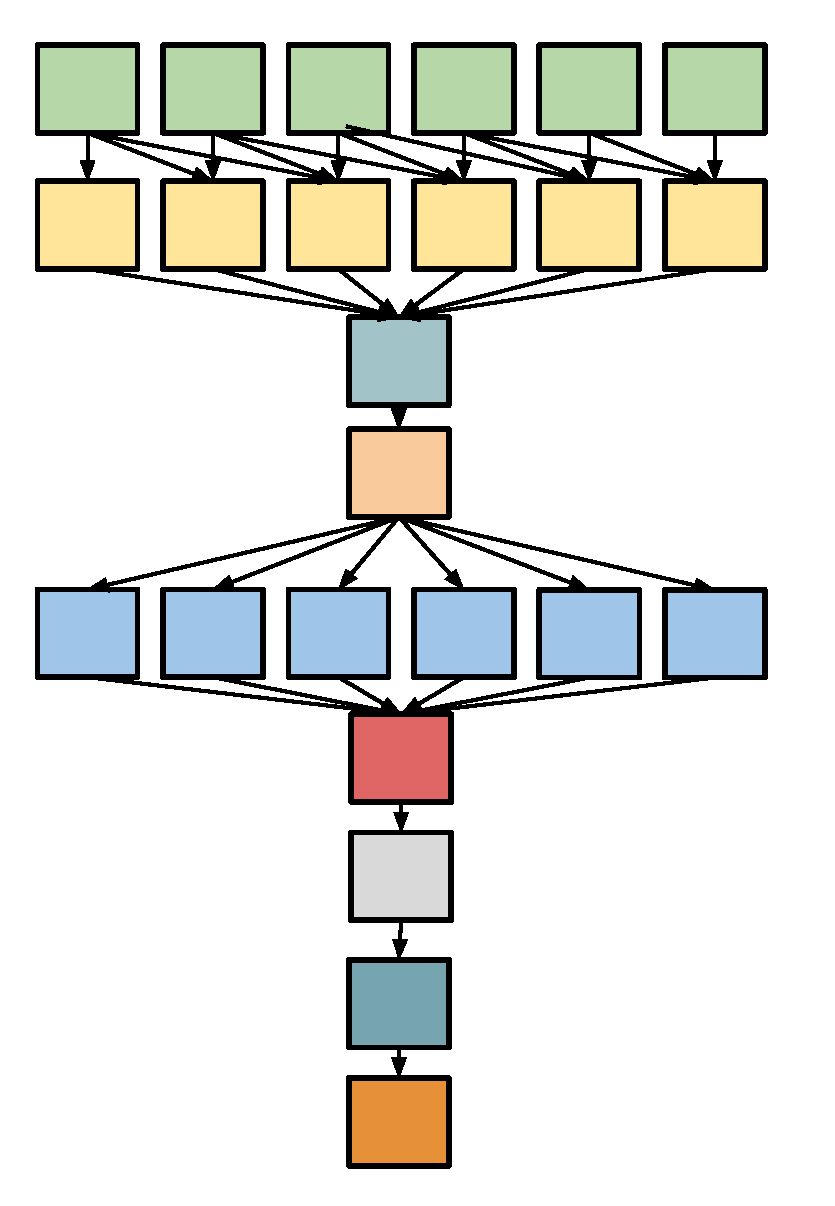
\includegraphics[width=0.38\linewidth]{montage_shape.pdf} \\
	\caption{Simplified visualization of the Montage workflow.}
	\label{fig:evaluation-shape-montage}
	\vspace{-15pt}
\end{figure}

\noindent \textbf{Cybershake.}
CyberShake~\cite{Graves2010} is a seismology application that calculates probabilistic seismic hazard 
curves for geographic sites in the Southern California region. It identifies all ruptures within 200km of the 
site of interest and converts rupture definition into multiple rupture variations with differing hypocenter 
locations and slip distributions. It calculates synthetic seismograms for each rupture variance from where 
peak intensity measures are extracted and combined with the original rupture 
probabilities to produce probabilistic seismic hazard curves for the site. Fig.~\ref{fig:evaluation-shape-cybershake} 
shows an illustration of the Cybershake workflow.

\begin{figure}[!htb]
	\centering
	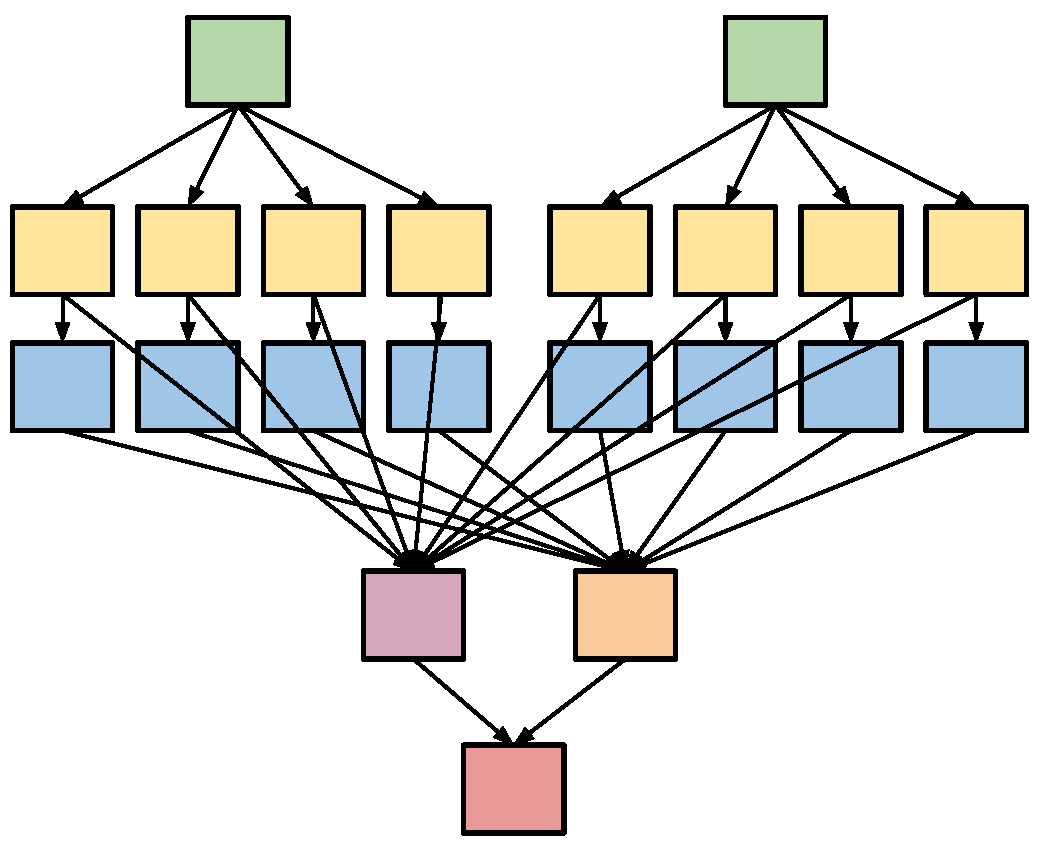
\includegraphics[width=0.53\linewidth]{cybershake_shape.pdf} \\
	\caption{Simplified visualization of the CyberShake workflow.}
	\label{fig:evaluation-shape-cybershake}
	\vspace{-10pt}
\end{figure}

\noindent \textbf{Epigenomics.}
The Epigenomics workflow~\cite{Epigenome} is a CPU-intensive application. Initial data are acquired 
from the Illumina-Solexa Genetic Analyzer in the form of DNA sequence lanes. Each Solexa machine 
can generate multiple lanes of DNA sequences. These data are converted into a format that can be used 
by sequence mapping software. The workflow maps DNA sequences to the correct locations in a reference 
Genome. Then it generates a map that displays the sequence density showing how many times a certain 
sequence expresses itself on a particular location on the reference genome. The simplified structure of 
Epigenomics is shown in Fig.~\ref{fig:evaluation-shape-genome}. 

\begin{figure}[!htb]
	\centering
	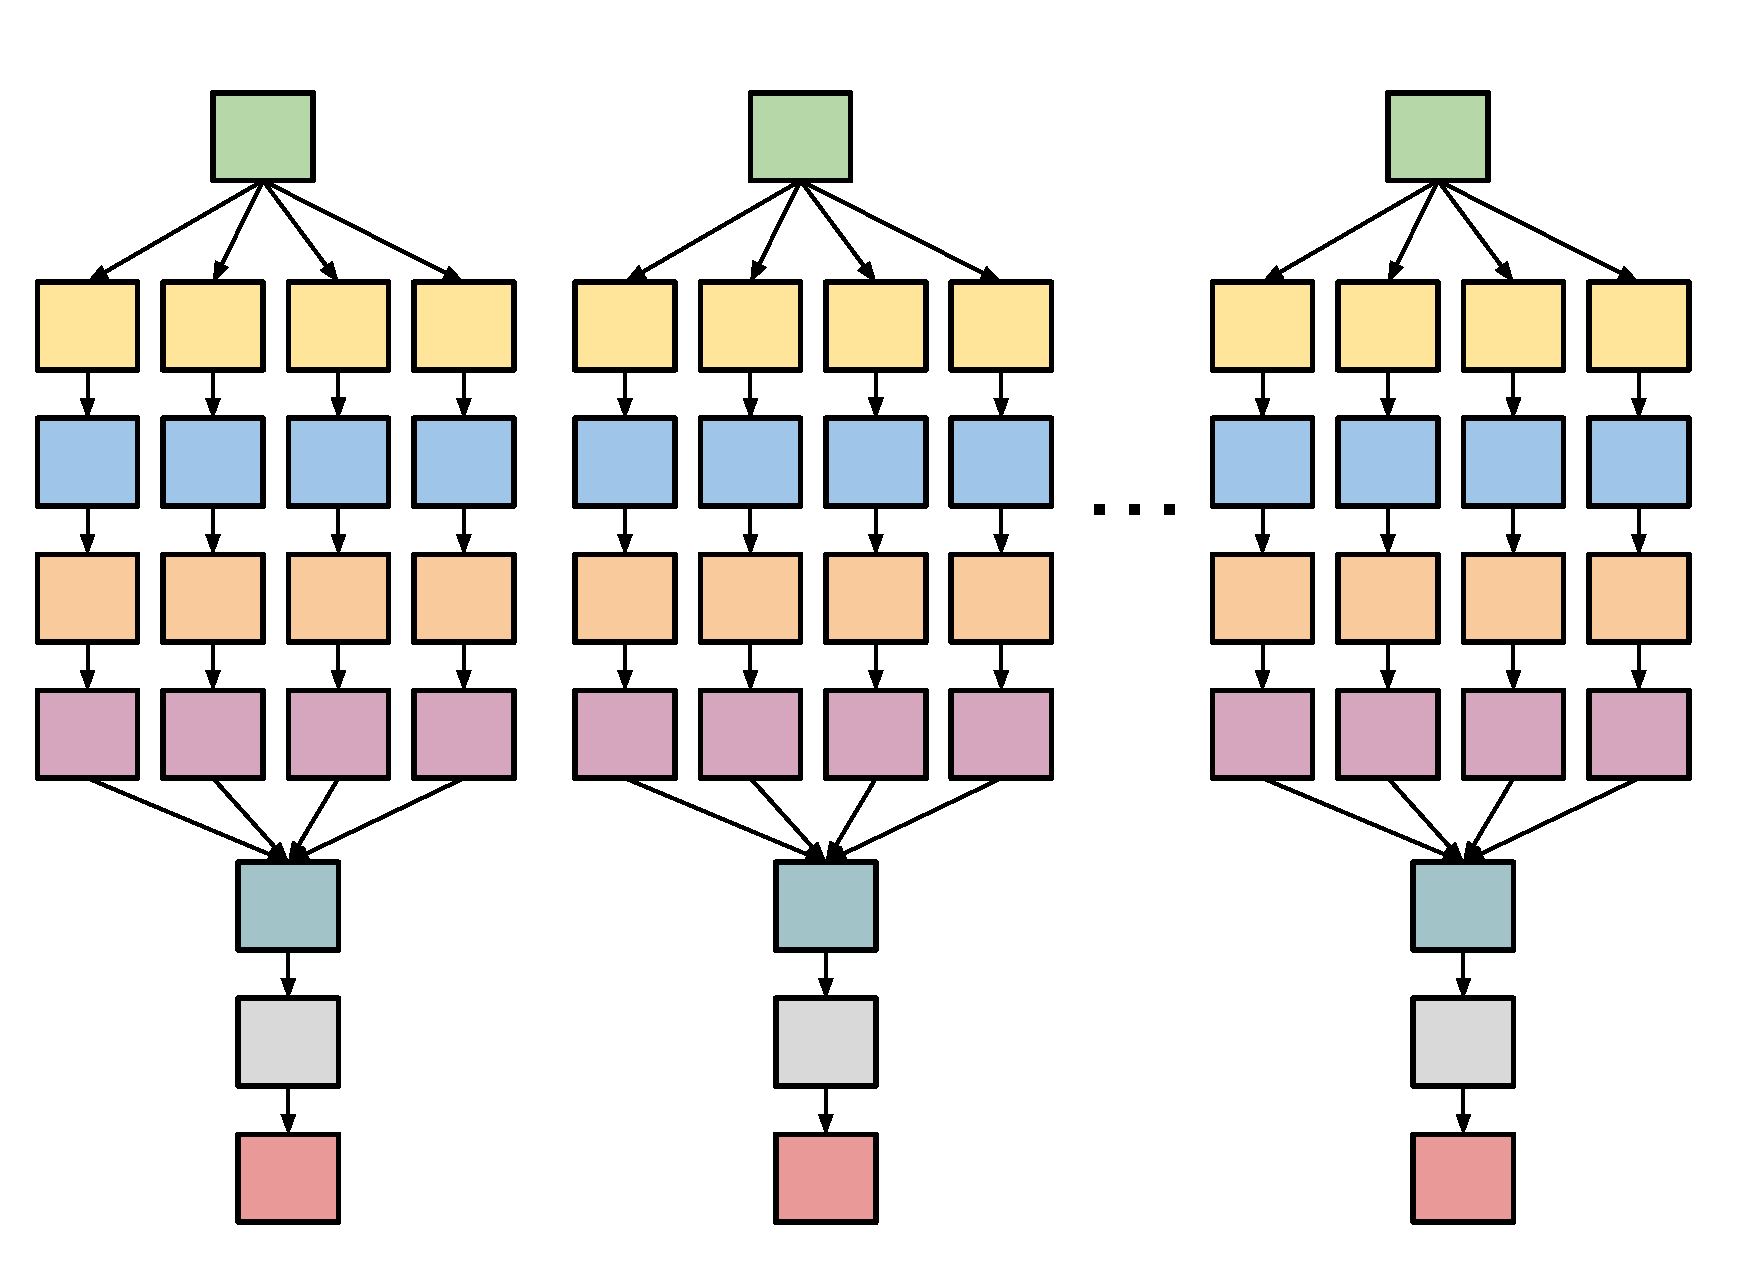
\includegraphics[width=0.8\linewidth]{genome_shape.pdf} \\
	\caption{Simplified visualization of the Epigenomics workflow with multiple branches.}
	\label{fig:evaluation-shape-genome}
	\vspace{-5pt}
\end{figure}

\noindent \textbf{SIPHT.}
The SIPHT workflow~\cite{SIPHT} conducts a wide search for small untranslated RNAs (sRNAs) that 
regulates several processes such as secretion or virulence in bacteria. The kingdom-wide prediction and 
annotation of sRNA encoding genes involves a variety of individual programs that are executed in the 
proper order using Pegasus~\cite{Deelman2005}. These involve the prediction of $\rho$-independent 
transcriptional terminators, BLAST (Basic Local Alignment Search Tools~\cite{BLAST}) comparisons 
of the inter genetic regions of different replicons and the annotations of any sRNAs that are found. 
A simplified structure of the SIPHT workflow is shown in Fig.~\ref{fig:evaluation-shape-sipht}. 

\begin{figure}[htb]
	\centering
	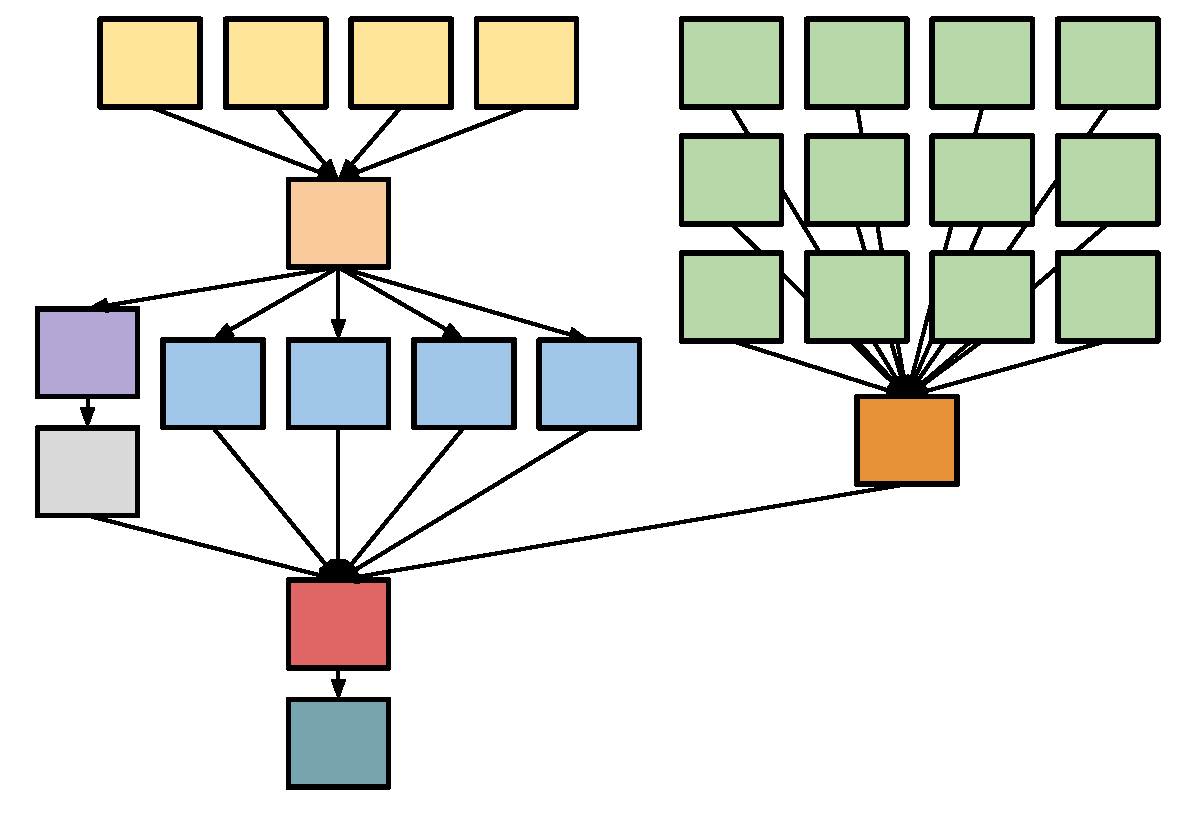
\includegraphics[width=0.55\linewidth]{sipht_shape.pdf} \\
	\caption{A simplified visualization of the SIPHT workflow.}
	\label{fig:evaluation-shape-sipht}
	\vspace{-5pt}
\end{figure}

Table~\ref{tab:evaluation-workflows} shows the summary of the main \emph{workflow characteristics}: 
number of tasks, average data size, and average task runtimes for the five workflows. 

\begin{table}[!htb]
	\setlength{\tabcolsep}{9pt}
	\centering
	\small
	\begin{tabular}{lrrrr}
		\hline
		 & \multicolumn{1}{c}{Number} & \multicolumn{1}{c}{Average} &  \multicolumn{1}{c}{Average} \\
		Workflow	& of Tasks	 & Data Size & Task Runtime \\
		\hline
		LIGO 		&800		& 5 MB	& 228s\\
		Montage 		&300		&3 MB	&11s\\
		CyberShake 	&700		&148 MB 	& 23s\\
		Epigenomics 	&165 	& 355 MB	& 2952s\\
		SIPHT		&1000	& 360 KB 	& 180s\\
		\hline
	\end{tabular}
	\caption{Summary of the main workflows characteristics.}
	\label{tab:evaluation-workflows}
	\vspace{-15pt}
\end{table} 


% Experiment conditions
\subsection{Experiment conditions}
\label{sec:experiment_conditions}

We adopt a trace-based simulation approach, where we extend our WorkflowSim~\cite{WorkflowSim} 
simulator with the fault-tolerant clustering methods to simulate a controlled distributed environment,
where system (i.e., the inter-arrival time of failures) and workflow (i.e., avg. task runtime) settings can
be varied to fully explore the performance of our fault-tolerant clustering algorithms.
WorkflowSim is an open source workflow simulator that extends CloudSim~\cite{Calheiros2011} by 
providing support for task clustering, task scheduling, and resource provisioning at the workflow level. 
It has been recently used in multiple workflow study areas~\cite{WorkflowSim,Chen2012, jrad2013broker} 
and its correctness has been verified in~\cite{WorkflowSim}.

The simulated computing platform is composed of 20 single homogeneous core virtual machines 
(worker nodes), which is the quota per user of some typical distributed environments such as Amazon 
EC2~\cite{AmazonAWS} and FutureGrid~\cite{FutureGrid}. 
%Amazon EC2 is a commercial, public cloud that has been widely used in distributed computing, in particular for scientific workflows~\cite{Berriman2010}. FutureGrid is a distributed, high-performance testbed that provides scientists with a set of computing resources to develop parallel, grid, and cloud applications. 
Each simulated virtual machine (VM) has 512MB of memory and the capacity to process 1,000 million 
instructions per second. The default network bandwidth is 15MB according to the execution environment 
in FutureGrid from where our traces were collected. By default, tasks at the same horizontal level 
are merged into 20 clustered jobs, which is a simple granularity control selection based on the strength 
of task clustering (as shown in~\cite{Chen2013b}).

We collected workflow execution traces~\cite{Juve2013, Chen2011} (including overhead and task 
runtime information) from real runs of the scientific workflow applications described in Section~\ref{sec:applications}. 
The traces are used to feed the Workflow Generator~\cite{rafael2014community} toolkit to generate 
synthetic workflows. The toolkit uses the information gathered from actual scientific workflow executions 
to generate synthetic workflows resembling those used by real world scientific applications. The number 
of inputs to be processed, the number of tasks in the workflow, and their composition determine the 
structure of the generated workflow. 

Three sets of experiments are conducted. Experiment 1 evaluates the performance of our fault-tolerant 
clustering methods (DR, VR, and SR) over an existing task clustering method (HC), which has no devoided 
of fault-tolerant mechanisms. The goal of the experiment is to identify conditions where each method works 
best and worst. We also evaluate the performance improvement for different $\theta_{\gamma}$ values 
(the inter-arrival time of task failures). $\theta_{\gamma}$ ranges from 1 to 10 times of the average task 
runtime such that the workflows do not run continuously and the performance difference is visually explicit. 

Experiment 2 evaluates the performance impact of the variation of the average task runtime per level 
(defined as the average of all the tasks per level) and the average system overheads per level for one 
scientific workflow application (CyberShake). In particular, we are interested in the performance of DR 
based on the results of Experiment 1. For this experiment, we use $\theta_{\gamma}=100$ since it 
better highlights the difference between the four methods. We vary the average task runtime of the 
CyberShake workflow (originally of about 23 seconds, Table~\ref{tab:evaluation-workflows}) by using 
a multiplier factor $f_r \in [0.5, 1.3]$. We also vary the average system overheads (originally of about 50 
seconds) by using a multiplier factor $f_o \in [0.2, 1.8]$.  

Experiment 3 evaluates the performance of the static and dynamic estimation. In the static estimation 
process, only the prior knowledge is used to estimate the MLEs of the unknown parameters. In contrast,
the dynamic estimation process leverages the runtime data collected during the execution and update 
the MLEs respectively. 

The experiments use two sets of the $\theta_{\gamma}$ function. The first is a step function 
(Fig.~\ref{fig:evaluation_step_signal}), in which $\theta_{\gamma}$ is decreased from 500 seconds 
to 50 seconds at time $T_d$. The step function of $\theta_{\gamma}$ at time $t_c$ is defined as follows:

\begin{equation}
	\label{eq:step_function}
	\theta_{\gamma}(t_c) =
	\begin{cases}
		50 & \text{if } t_c \geq T_d \\
		500       & \text{if } 0< t_c < T_d
	\end{cases}
\end{equation}
This function simulates a scenario where failures happen more frequently than expected. We evaluate 
the performance difference of dynamic and static estimations for $1000 \leq T_d \leq 5000$ based on 
the estimation of the workflow makespan. Theoretically speaking, the later we change $\theta_{\gamma}$, 
the less the re-clustering is influenced by the estimation error, and thus the smaller the workflow makespan 
is. There is one special case when $T_d\to 0$, which means the prior knowledge is wrong at the very 
beginning.

\begin{figure}[!htb]
	\centering
	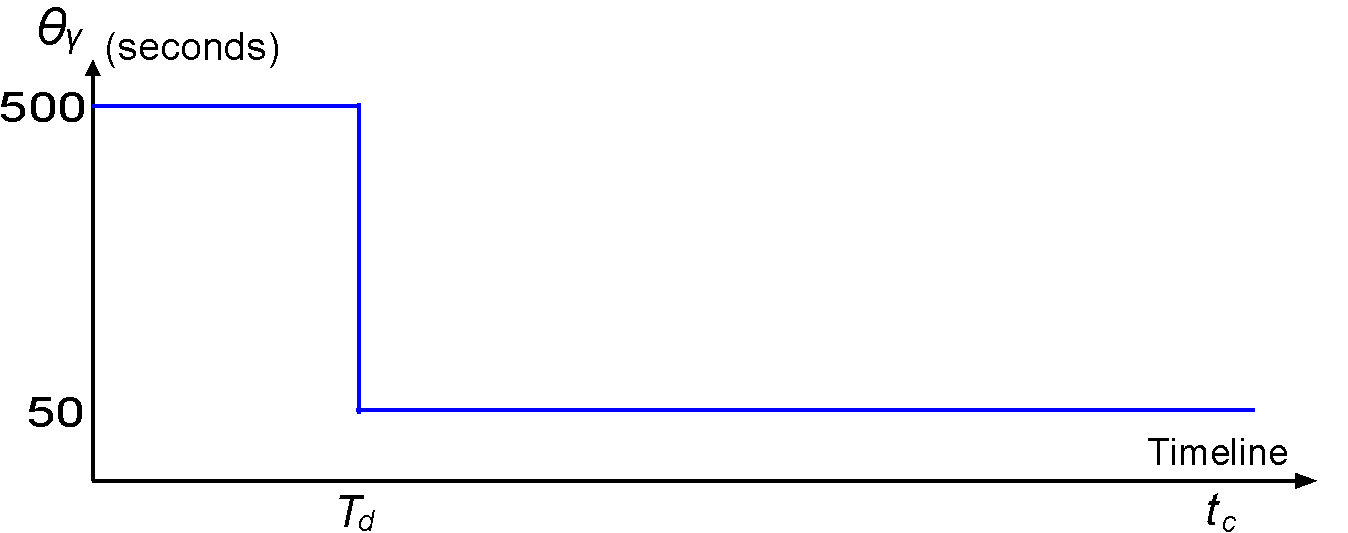
\includegraphics[width=0.8\linewidth]{step_signal.pdf} \\
	\caption{A Step Function of $\theta_{\gamma}$. $t_c$ is the current time and $T_d$ is the moment $\theta_{\gamma}$ changes from 500 to 50 seconds.}
	\label{fig:evaluation_step_signal}
	\vspace{-10pt}
\end{figure}

The second function is a pulse wave function (Fig. \ref{fig:evaluation_pulse_signal}) in which the 
amplitude alternates at a steady frequency between a fixed minimum (50 seconds) to a maximum 
(500 seconds) value. The function is defined as follows:

\begin{equation}
	\label{eq:pulse_function}
	\theta_{\gamma}(t_c) =
	\begin{cases}
		500 & \text{if } 0< t_c \leq \tau \\
		50       & \text{if } \tau< t_c < T_c
	\end{cases}
\end{equation}
where $T_c$ is the period, and $\tau$ is the duty cycle of the oscillator. This function simulates a 
scenario where the failures follow a periodic pattern~\cite{yigitbasi2010analysis} extracted from 
failure traces obtained from production distributed systems. In this work, we vary $T_c$ from 
1000 seconds to 10000 seconds based on the estimation of the workflow's makespan, and 
$\tau$ from $0.1T_c$ to $0.5T_c$. 

\begin{figure}[!htb]
	\centering
	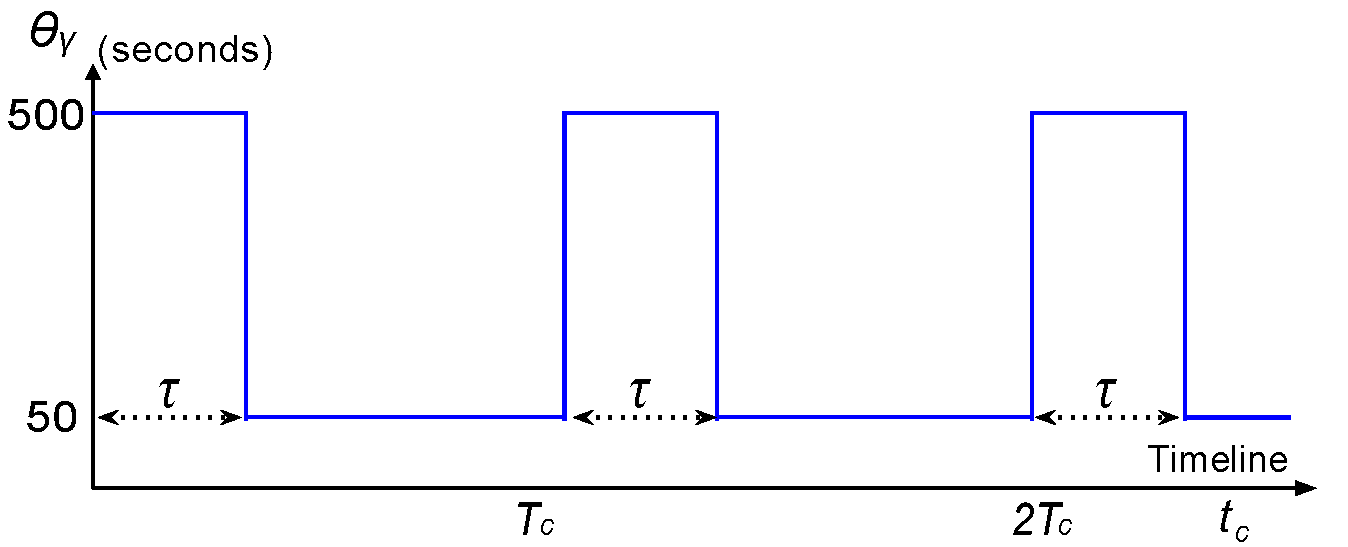
\includegraphics[width=0.8\linewidth]{pulse_signal.pdf} \\
	\caption{A Pulse Function of $\theta_{\gamma}$. $t_c$ is the current time and $T_c$ is the period of the wave. $\tau$ is the width of the pulse.}
	\label{fig:evaluation_pulse_signal}
	\vspace{-15pt}
\end{figure}

%Table~\ref{tab:evaluation_methods} summarizes the task clustering methods to be evaluated in 
%our experiments. 
%
%\begin{table}[!htb]
%	\setlength{\tabcolsep}{10pt}
%	\centering
%	\small
%	\begin{tabular}{c l}
%		\hline
%		Abbreviation	& Method	  \\ \hline
%		DR 			& Dynamic Reclustering \\
%		SR 			&Selective Reclustering \\
%		VR 			&Vertical Reclustering \\
%		HC 			&Horizontal Clustering \\
%		\hline
%	\end{tabular}
%	\caption{Task clustering methods used in the experiements.}
%	\label{tab:evaluation_methods}
%\end{table} 


% Results and Discussion
\subsection{Results and Discussion}
\label{sec:results}

\begin{figure}[!t]
	\centering
	
	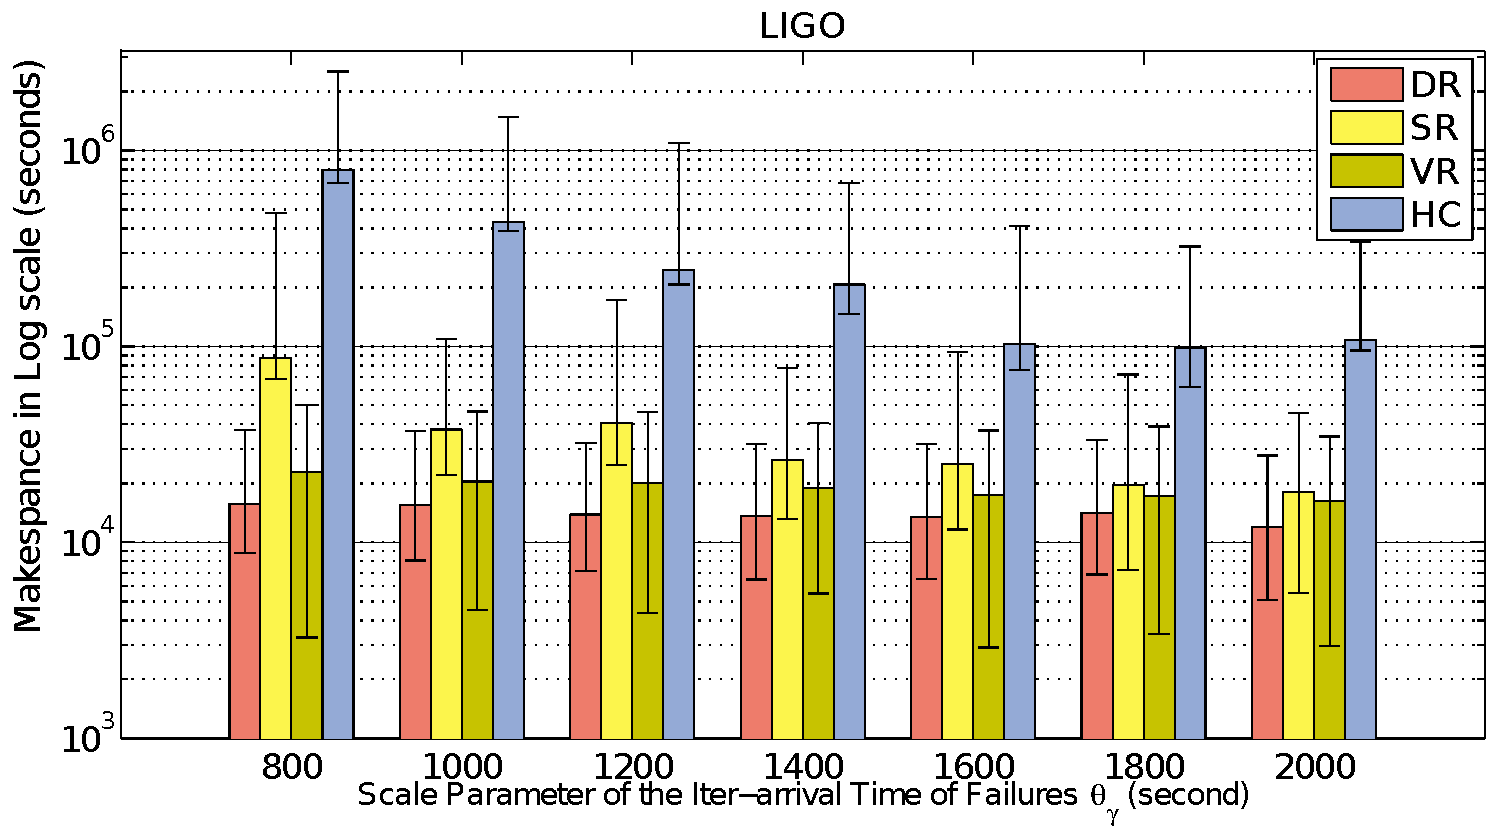
\includegraphics[width=.836\linewidth]{ligo} \\
	\small (a) LIGO workflow \\ \vspace{3pt}
	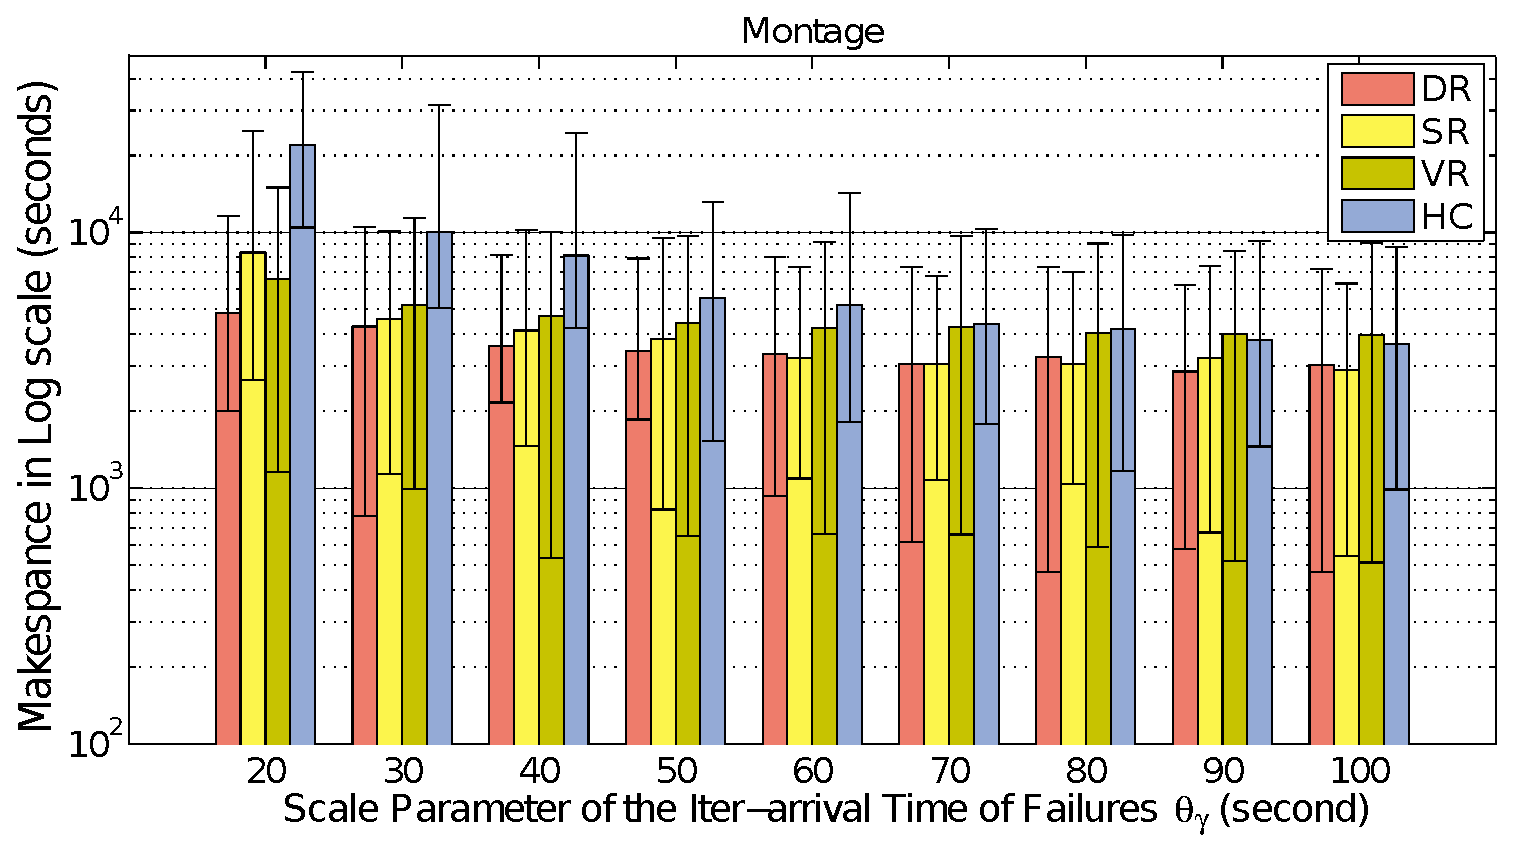
\includegraphics[width=.836\linewidth]{montage} \\
	\small (b) Montage workflow \\ \vspace{3pt}
	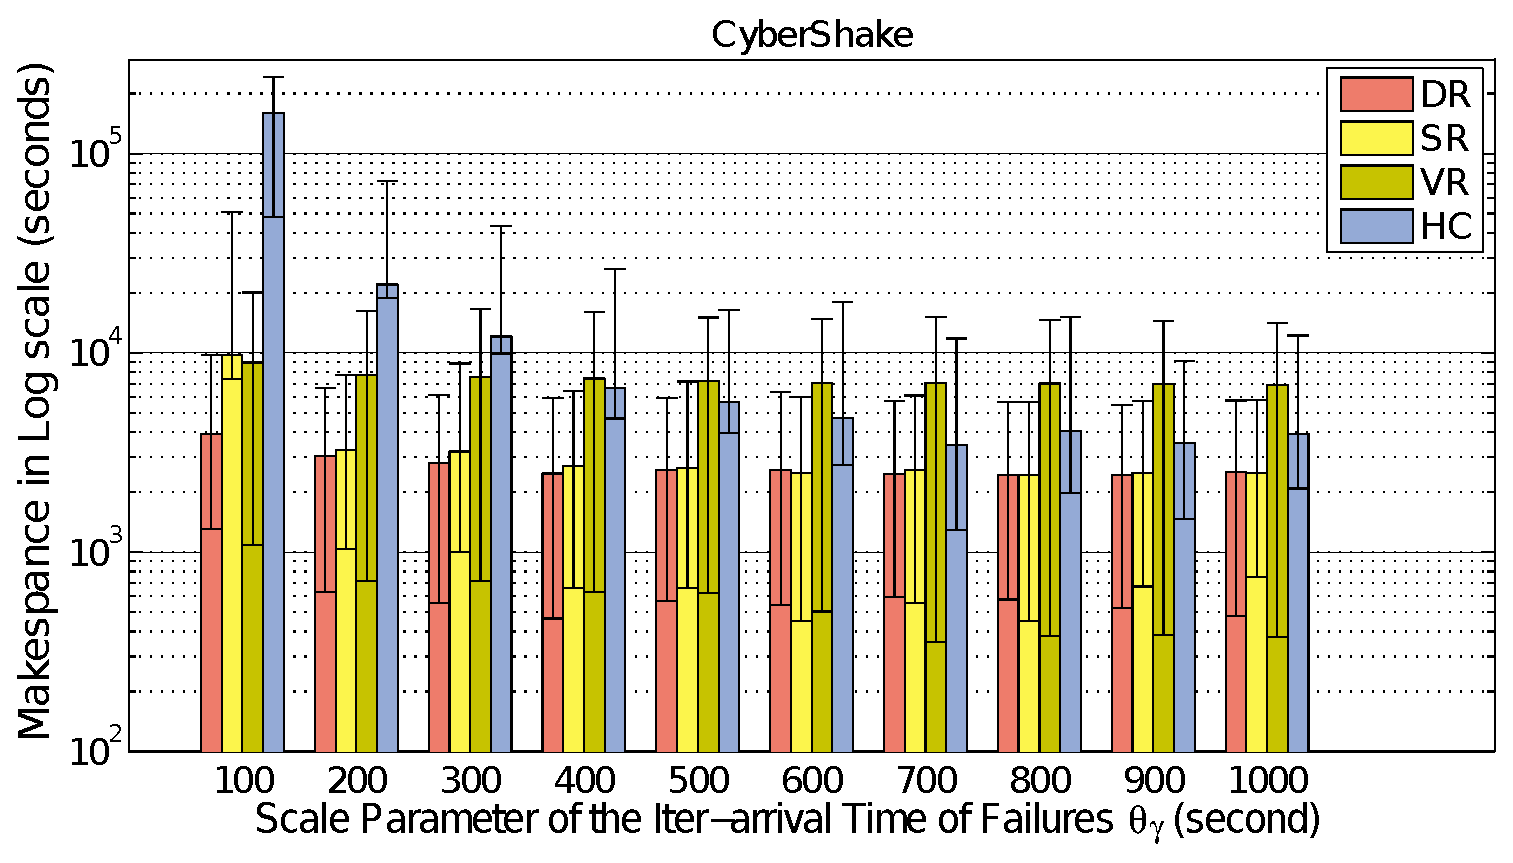
\includegraphics[width=.836\linewidth]{cybershake} \\
	\small (c) CyberShake workflow \\ \vspace{3pt}
	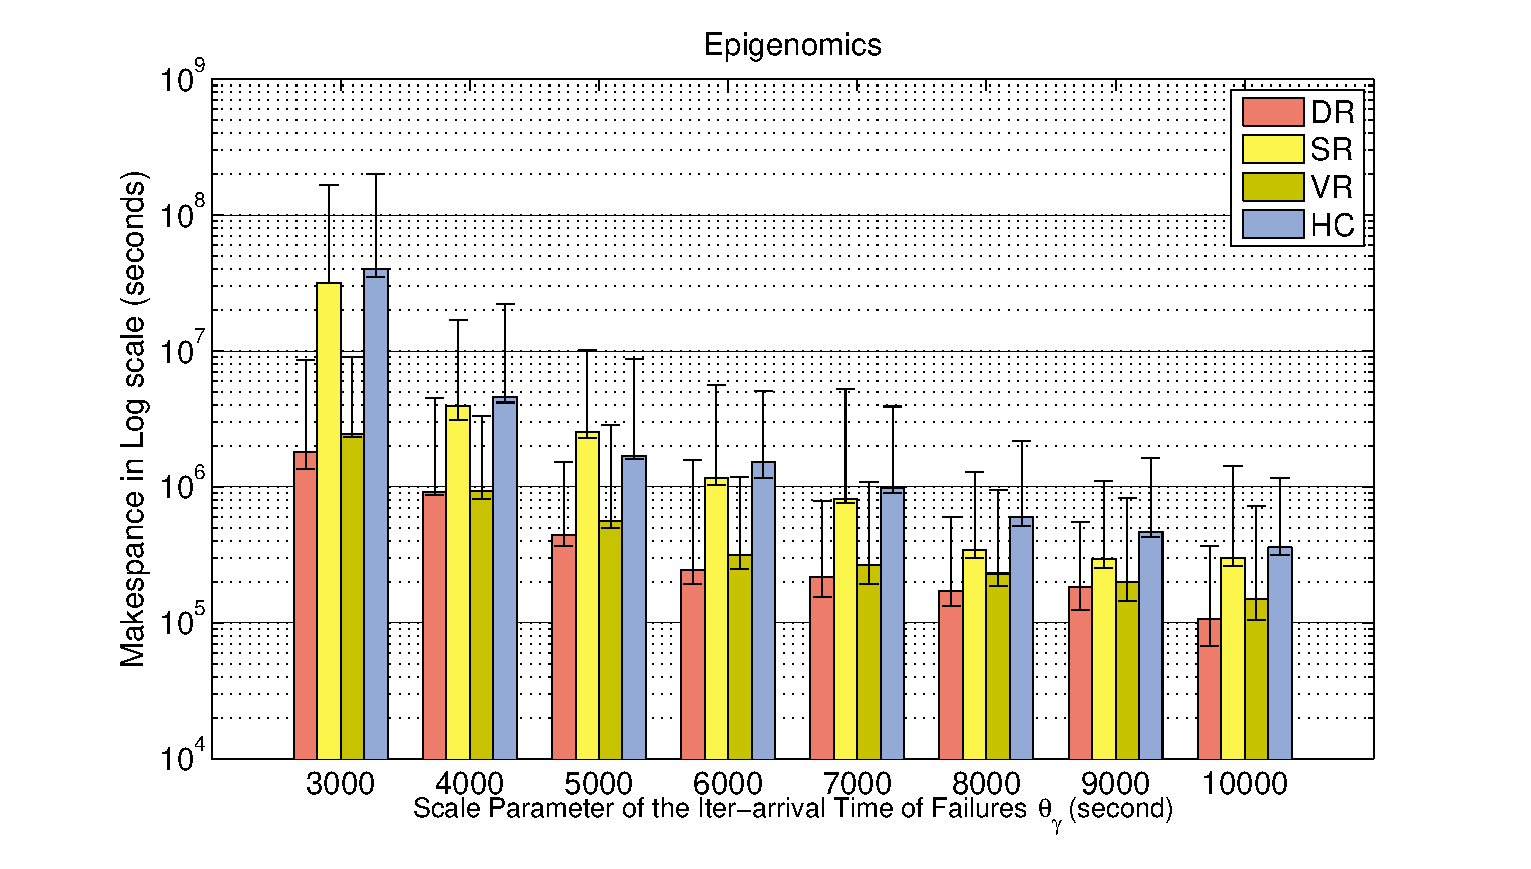
\includegraphics[width=.836\linewidth]{genome} \\
	\small (d) Epigenomics workflow \\ \vspace{3pt}
	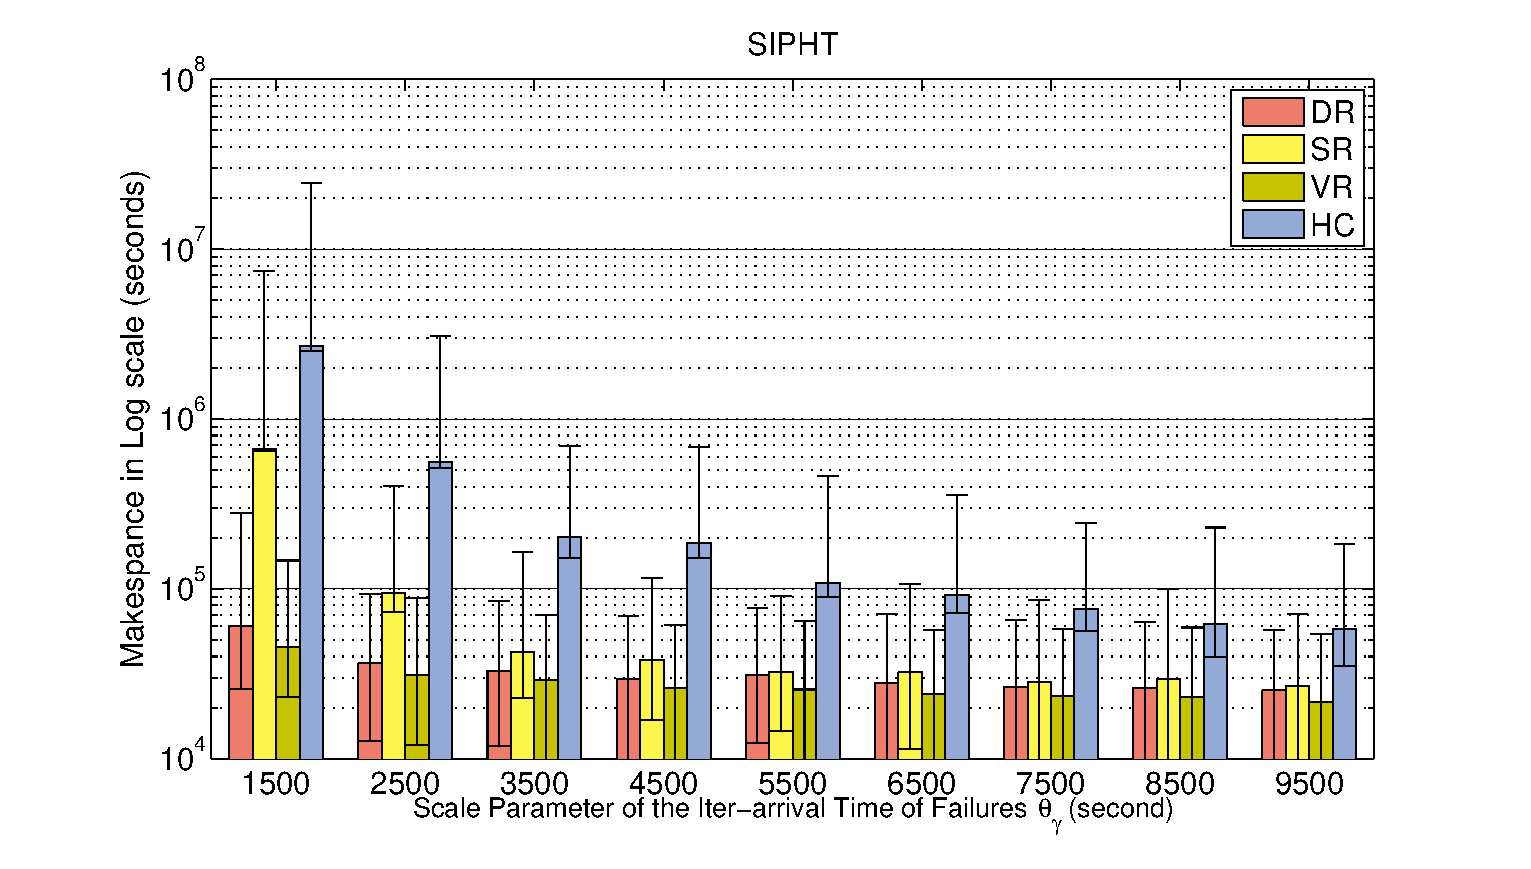
\includegraphics[width=.836\linewidth]{sipht} \\
	\small (e) SIPHT workflow \\ \vspace{3pt}
	
	\caption{(\emph{Experiment 1}): Performance evaluation of our fault-tolerant task clustering methods for different values of the inter-arrival time~($\theta_{\gamma}$).}
  \label{fig:exp1}
\end{figure}

\noindent \textbf{Experiment 1.}
Fig.~\ref{fig:exp1} shows the performance of the Horizontal Clustering (HC), Selective 
Reclustering (SR), Dynamic Reclustering (DR), and Vertical Reclustering (VR) methods 
for the five workflows. DR, SR, and VR significantly improve the makespan when compared 
to HC in a large scale. By decreasing of the inter-arrival time~($\theta_{\gamma}$) and 
consequently generating more task failures, the performance improvement for our fault-tolerant 
task clustering methods becomes more significant. Among the three methods, DR and VR 
perform consistently better than SR, which fails to improve the makespan when $\theta_{\gamma}$ 
is small. The reason is that SR does not adjust $k$ according to the occurrence of failures. 

The performance of VR is tightly coupled to the workflow structure and the average task runtime. 
For example, according to Fig.~\ref{fig:evaluation-shape-genome} and Table~\ref{tab:evaluation-workflows}, 
the Epigenomics workflow has a long task runtime (around 50 minutes) and the pipeline length is 4. 
This means that vertical clustering creates very long jobs ($\sim50 \times 4 = 200$ minutes) and 
thereby VR is more sensitive to the decrease of $\gamma$. As indicated in Fig.~\ref{fig:exp1}.d, 
the makespan increases more significantly with the decrease of $\theta_{\gamma}$ than for other 
workflows. In contrast, vertical clustering does not improve makespan in the CyberShake workflow 
(Fig.~\ref{fig:exp1}.c) since it does not have many pipelines (Fig.~\ref{fig:evaluation-shape-cybershake}). 
In addition, the average task runtime of the CyberShake workflow is relatively short (around 23 
seconds). Compared to horizontal clustering methods such as HC, SR and DR, vertical clustering 
does not generate long jobs and thus the performance of VR is less sensitive to $\theta_{\gamma}$. 

%4). Under some cases, i.e., the CyberShake workflow, we see that VR does not perform well compared to DR or SR. The reason is the graph structure of the CyberShake workflow does not leave much space for vertical clustering methods to improve since it does not have many pipelines as shown in Figure~\ref{fig:evaluation_shape_cybershake}. DR, a modification of HC, is more likely to improve the performance since most of these workflows have many parallel tasks in the same level. 

\begin{figure}[t]
	\centering
	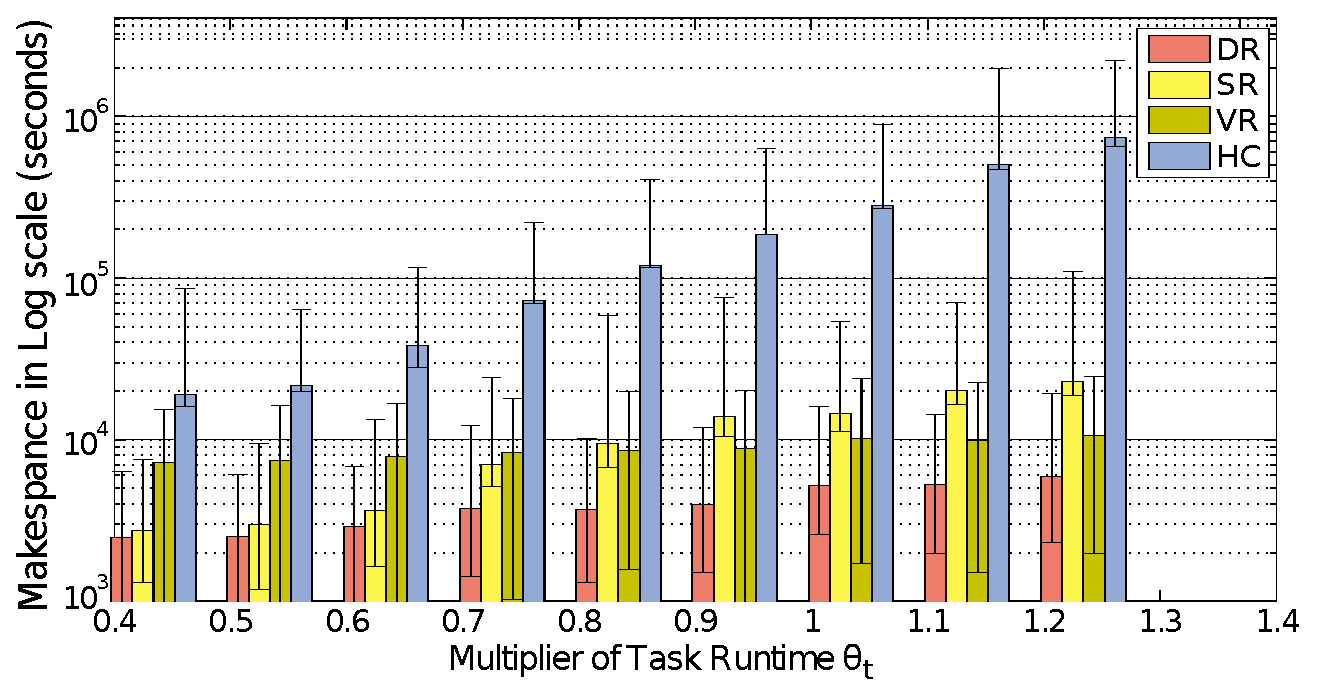
\includegraphics[width=1\linewidth]{t.eps}
	\caption{(\emph{Experiment 2}): Influence of varying task runtime ($\theta_t$) on makespan for the CyberShake workflow.}
	\label{fig:expr_t}
	\vspace{-15pt}
\end{figure}

\begin{figure}[!t]
	\centering
	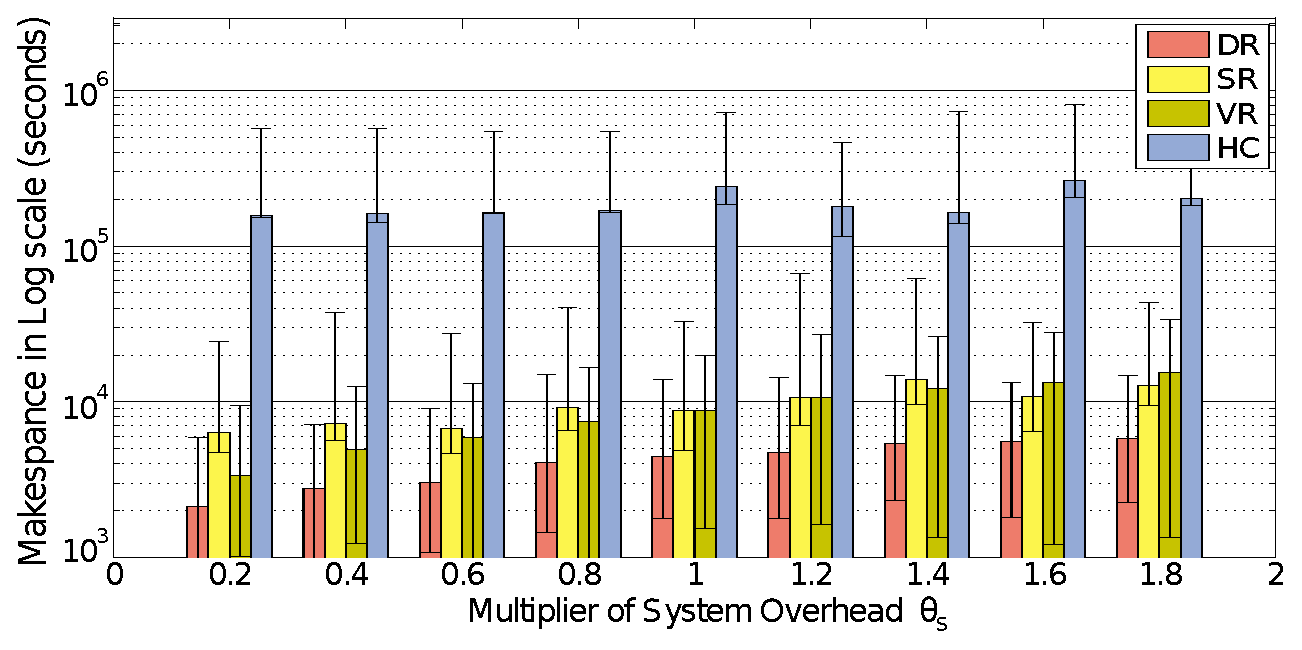
\includegraphics[width=1\linewidth]{d.eps}
	\caption{(\emph{Experiment 2}): Influence of varying system overhead ($\theta_s$) on makespan for the CyberShake workflow.}
	\label{fig:expr_d}
	\vspace{-15pt}
\end{figure}

\vspace{5pt}
\noindent \textbf{Experiment 2.}
Fig.~\ref{fig:expr_t} shows the performance (CyberShake workflow) of the task clustering 
methods,  when the task runtime is varied by a multiplier factor $\theta_{t}$. 
By increasing the task runtime, HC has the most negative impact on the workflow's makespan 
(increase from a scale of $10^4$ to $\sim10^6$). This is due to the lack of fault-tolerant mechanisms,
since HC retries the entire clustered job. SR and VR, however, retry only failed tasks that are 
merged into a new clustered job. Although the selective and vertical methods 
significantly speedup the execution when compared to HC, they have no mechanism to
adjust the clustering size to the actual optimal clustering size, which may be larger or smaller
than the number of failed tasks. By dynamically adjusting the clustering size, DR yields better
makespans, in particular for high values of $\theta_t$.

Fig.~\ref{fig:expr_d} shows the performance (for the CyberShake workflow) of the task clustering 
methods methods,  when the system overhead is varied by using a multiplier factor $\theta_s$. 
Similarly, with the increase of the system overhead, HC is significantly impacted while SR and VR 
perform better. Again, for high $\theta_s$ values DR performs best. Note that the improvement 
yielded by the fault-tolerant methods is less significant than the performance improvements shown
in Fig.~\ref{fig:expr_t}. The reason is that clustered jobs may have multiple tasks but only one 
system overhead per job.

\vspace{5pt}
\noindent \textbf{Experiment 3.}
Fig.~\ref{fig:expr_static_dynamic} shows the performance evaluation of the dynamic and static estimations 
for the CyberShake workflow with a step function of $\theta_{\gamma}$. In this experiment, we use DR
as the fault-tolerant task clustering method since it yielded the best performance in the past  
experiments. The step signal function changes the inter-arrival time of failures ($\theta_\gamma$)
from 500 to 50 seconds at time $T_d$. For high values of $T_d$, failures are scarce since
the inter-arrival time is close to the workflow makespan. Therefore, the influence of $\theta_\gamma$ is
negligible, and thus both the static and dynamic estimations have the same behavior. When failures are
more frequent, i.e., low values for $T_d$, the dynamic estimation improves the workflow's makespan 
by up to 22\%. This improvement is due to the ability of the dynamic estimation process to update the 
MLEs of $\theta_{\gamma}$ and adapt the clustering size. 

\begin{figure}[t]
	\centering
	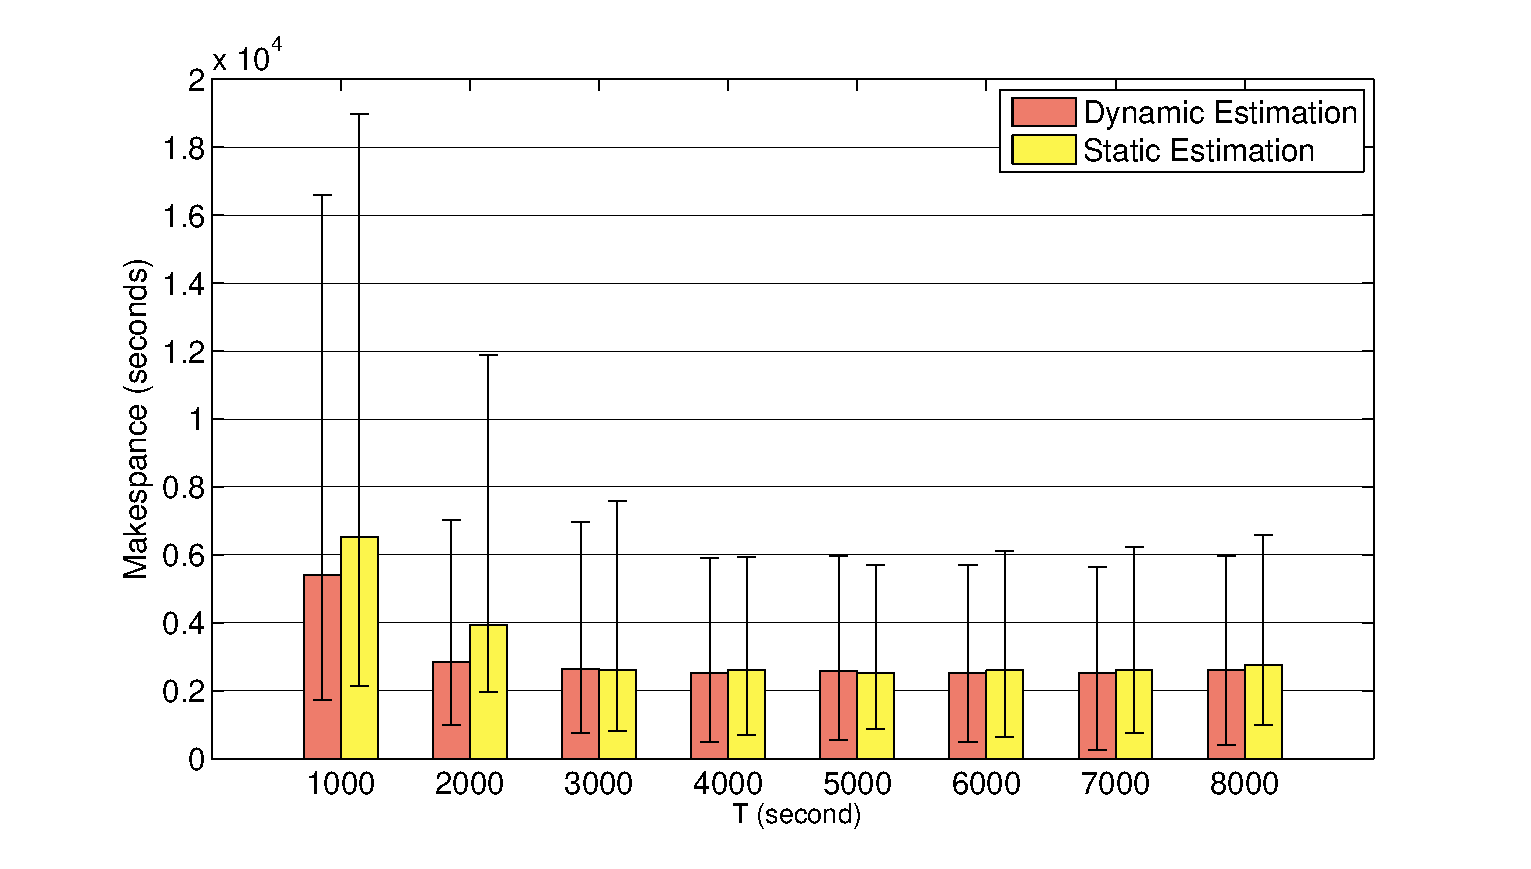
\includegraphics[width=\linewidth]{versus.eps}
	\caption{(\emph{Experiment 3}): Performance evaluation of the static and dynamic estimations for the CyberShake workflow using a step function.}
	\label{fig:expr_static_dynamic}
	\vspace{-5pt}
\end{figure}

\begin{figure}[!t]
	\centering
	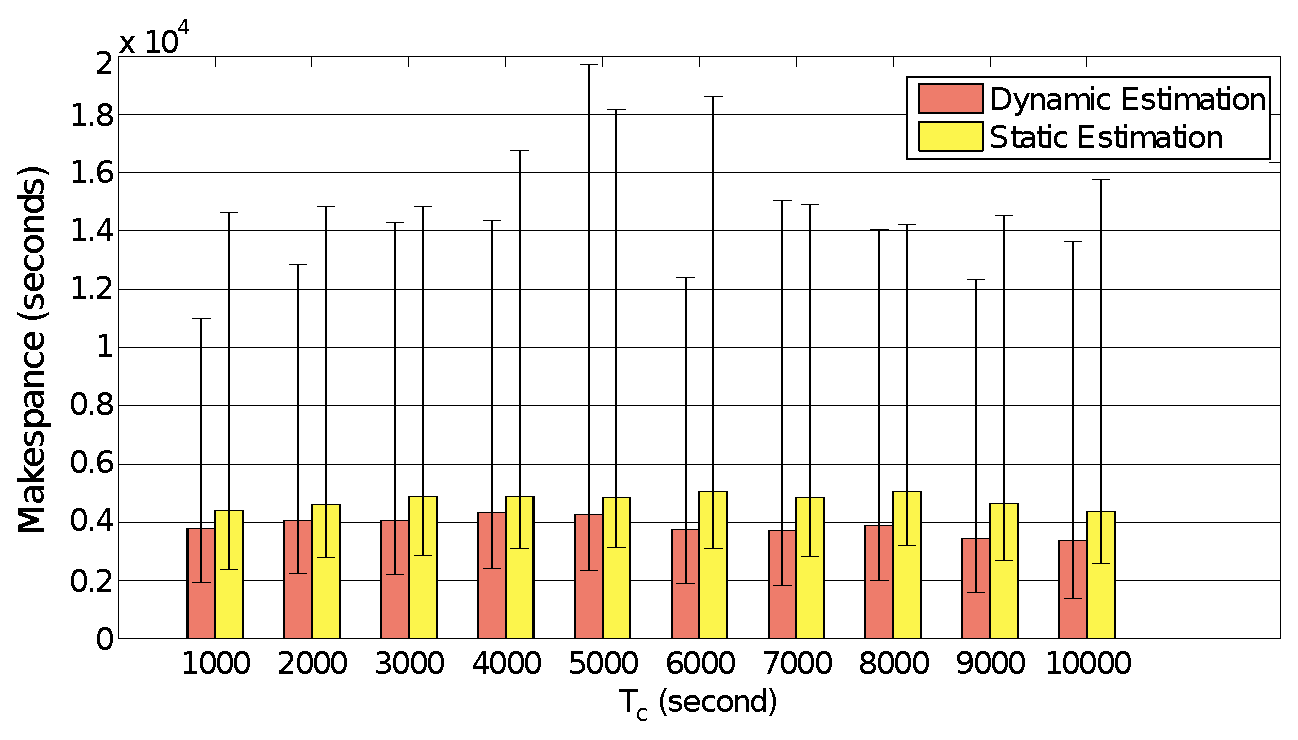
\includegraphics[width=1\linewidth]{pulse_t10.eps} \\
	\small (a) $\tau=0.1 \cdot T_c$ \\ \vspace{4pt}
	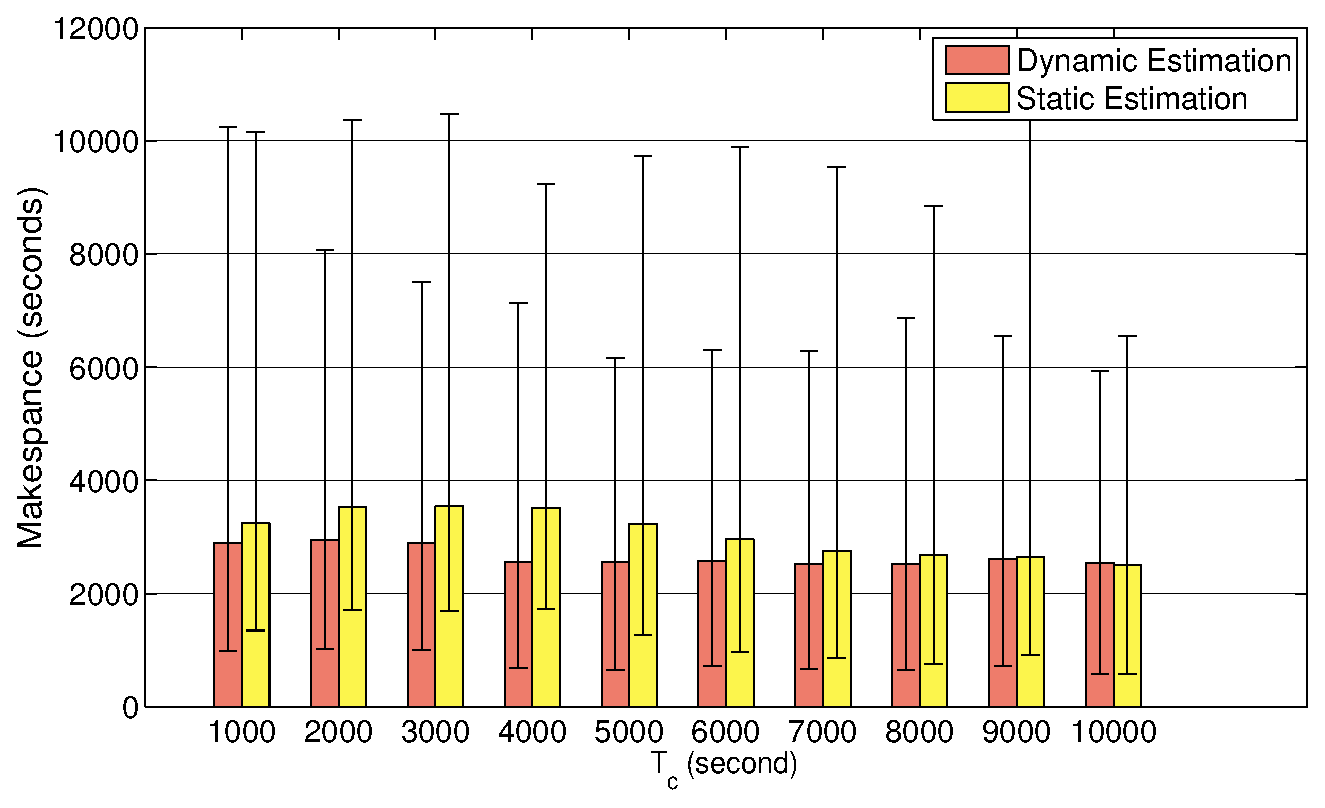
\includegraphics[width=1\linewidth]{pulse_t30.eps} \\
	\small (b) $\tau=0.3 \cdot T_c$ \\ \vspace{4pt}
	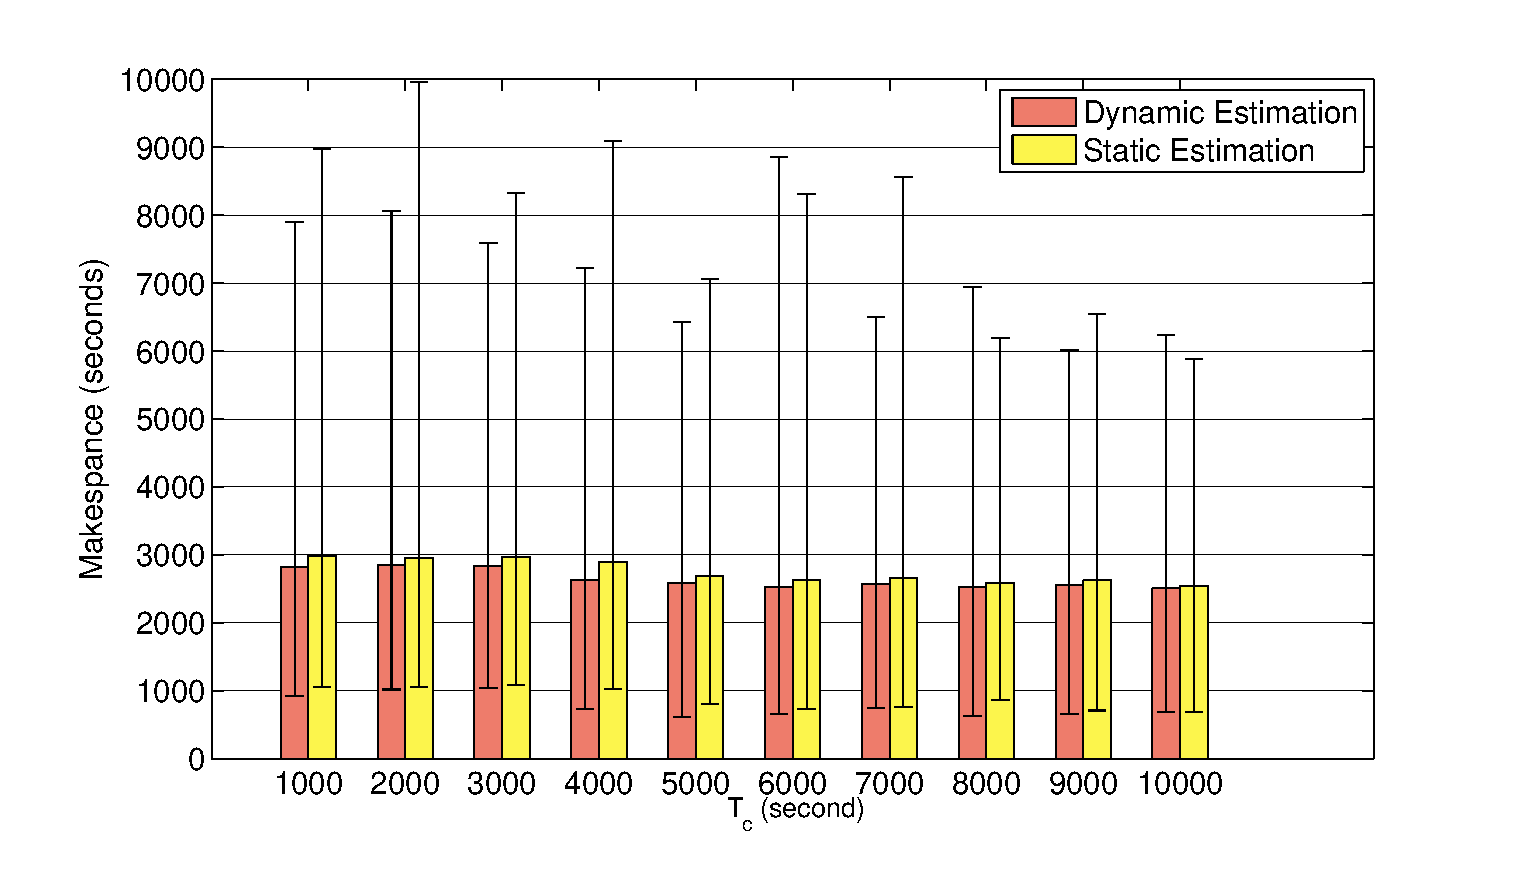
\includegraphics[width=1\linewidth]{pulse_t50.eps} \\
	\small (c) $\tau=0.5 \cdot T_c$
	\caption{(\emph{Experiment 3}): Performance evaluation of the static and dynamic estimations for the CyberShake workflow using a step function pulse function.}
	\label{fig:exp3}
	\vspace{-20pt}
\end{figure}


Fig.~\ref{fig:exp3} shows the performance evaluation of the dynamic and static estimations 
with a pulse function of $\theta_{\gamma}$. For this experiment,
we use $\tau = 0.1 \cdot T_c$, $0.3 \cdot T_c$, $0.5 \cdot T_c$ (Equation~\ref{eq:pulse_function}).
For $\tau = 0.1 \cdot T_c$ (Fig.~\ref{fig:exp3}.a), the dynamic estimation improves the makespan by up 
to 25.7\% compared to the static estimation case. For $\tau=0.3 \cdot T_c$ (Fig.~\ref{fig:exp3}.b), 
the performance gain of dynamic estimation over static estimation is up to 27.3\%. For $T_c = 1000$, 
the performance gain is not significant since the inter-arrival time of failures changes frequently and 
then the dynamic estimation process is not able to update swiftly. For $T_c = 10000$, the performance 
difference is not significant neither since the inter-arrival time is close to the makespan. For 
$\tau = 0.5 \cdot T_c$, the performance gain of dynamic over static estimation is not significant
and nearly constant (up to 9.1\%) since $\theta_{\gamma}$ has equal influence on the failure occurrence
regardless of its value. 




%
% Section: Conclusion and Future Work
%
\section{Conclusion and Future Work}

In this work, we model transient failures in a distributed environment and assess their influence 
on task clustering. We propose three dynamic clustering methods to improve the fault tolerance 
of task clustering and apply them to five widely used scientific workflows. Experimental results 
show that the proposed methods significantly improve the workflow's makespan when compared 
to an existing task clustering method used in workflow management systems. In particular, the 
Dynamic Reclustering method performs best among all methods since it can adjust the clustering 
size based on the Maximum Likelihood Estimation of task runtime, system overheads, and the 
inter-arrival time of failures. The Vertical Reclustering method significantly improves the performance 
for  workflows that have short task runtimes. The dynamic estimation process, which uses data 
collected during the workflow execution, can further improve the overall runtime in a dynamic 
environment where the inter-arrival time of failures is fluctuant.

This work is focused on the evaluation of fault-tolerant task clustering techniques on homogeneous 
environments. In the future, we plan to combine our work with fault-tolerant scheduling in heterogeneous 
environments, i.e, a scheduling algorithm that avoids mapping clustered jobs to failure-prone nodes. 
We also intend to combine vertical clustering methods with horizontal clustering methods. For example, 
vertical clustering can be performed either before or after horizontal clustering, which we believe would 
bring different performance improvement. 
%Our dynamic estimation using on-going data collected from the workflow execution can further improve the fault tolerance in a dynamic environment where the inter-arrival time of failures is fluctuant. 

We assume that the inter-arrival time of transient failures is a function of task type, which is one of 
the major impact factors. In the future, we plan to consider other major factors such as the execution 
site, which may improve the accuracy of the model. 



% use section* for acknowledgement
\ifCLASSOPTIONcompsoc
  % The Computer Society usually uses the plural form
  \section*{Acknowledgments}
\else
  % regular IEEE prefers the singular form
  \section*{Acknowledgment}
\fi

\footnotesize
This work was supported by NFS under grant number IIS-0905032. We thank Gideon Juve, 
Karan Vahi, Mats Rynge, and Rajiv Mayani for their valuable help. Traces are collected from 
experiments conducted on FutureGrid, which is supported by NSF under grant FutureGrid 0910812. 




\bibliographystyle{elsarticle-num}
\bibliography{biblio}

\begin{IEEEbiography}[{
\includegraphics[width=1in,height=1.25in,clip,keepaspectratio]{weiwei.eps}}]{Weiwei Chen} is a Ph.D. candidate in the Dept. of Computer Science, University of Southern California, USA. In 2009, he completed his bachelor in the Dept. of Automation, Tsinghua University, China. He is currently working on task clustering in scientific workflows. His research interests include distributed computing, services computing and data analysis. 
\end{IEEEbiography}
% insert where needed to balance the two columns on the last page with
% biographies
%\newpage



\begin{IEEEbiography}[{
\includegraphics[width=1in,height=1.25in,clip,keepaspectratio]{rafael.eps}}]{Rafael Ferreira da Silva} is a Computer Scientist at the USC Information Sciences Institute. He received his PhD in Computer Science from INSA-Lyon, France, in 2013. His research focuses on the optimization of the execution of scientific workflows on heterogeneous distributed systems. See http://www.rafaelsilva.com for further information.
\end{IEEEbiography}

%\newpage

\begin{IEEEbiography}[{\includegraphics[width=1in,height=1.25in,clip,keepaspectratio]{deelman.eps}}]{Ewa Deelman} is a Research Associate Professor at the USC Computer Science Department and a Assistant Division Director at the USC Information Sciences Institute. Her research interests include the design and exploration of distributed scientific environments, with emphasis on workflow management. She received her PhD in Computer Science from the Rensselaer Polytechnic Institute in 1997. 
\end{IEEEbiography}


\begin{IEEEbiography}[{
\includegraphics[width=1in,height=1.25in,clip,keepaspectratio]{thomas.eps}}]{Thomas Fahringer} received the Ph.D. degree in 1993 from the Vienna University of Technology. Since 2003, he has been a full professor of computer science in the Institute of Computer Science, University of Innsbruck, Austria. His main research interests include software architectures, programming paradigms, compiler technology, performance analysis, and prediction for parallel and distributed systems. 
\end{IEEEbiography}


\end{document}
